\documentclass[]{spie} % US letter paper
%\documentclass[a4paper]{spie} % A4 paper
%\documentclass[nocompress]{spie} % no compression of citations
\renewcommand{\baselinestretch}{1.0} % 1.65 for double spacing 
\usepackage{amsmath,amsfonts,amssymb}
\usepackage{graphicx}
\usepackage{wrapfig}
\usepackage{csquotes}
\usepackage{xcolor}
\usepackage{framed}
\usepackage{soul}
\usepackage{float}
\usepackage{stackengine}
\usepackage{gensymb}
\usepackage{booktabs}
% \usepackage{lipsum}
\usepackage{colortbl}
\usepackage[colorlinks=true, allcolors=blue]{hyperref}

\definecolor{tablegrey}{HTML}{808080}

% style
\pagestyle{empty}
%\pagestyle{plain} % for page numbers
%\setcounter{page}{301} % start numbering at 301
%\sethlcolor{green} % default highlighter
%\definecolor{example}{RGB}{28, 69, 135} % custom color
%\colorlet{shadecolor}{orange}

% macros
\DeclareQuoteStyle[american]{english}{\itshape\textquotedblleft}[\textquotedblleft]{\textquotedblright}[0.05em]{\textquoteleft}{\textquoteright}
\DeclareRobustCommand{\hlnote}[1]{{\sethlcolor{green}\hl{\textsc{#1}}}}
\DeclareRobustCommand{\framenote}[1]{{\colorlet{shadegreen}{yellow}\begin{shaded}#1\end{shaded}}}

% title
\title{Learning and estimating whole sky visible, VNIR, SWIR radiance distributions from a commercial camera}

% authors
\author[a]{Joseph Del Rocco}
\author[b]{Charles Brandon Patterson}
\author[c]{Hassen Dhrif}
\author[a]{Joseph T. Kider Jr.}
\affil[a]{Institute for Simulation and Training, University of Central Florida, Orlando, FL, USA}
\affil[b]{Full Sail University, Winter Park, FL, USA}
\affil[c]{University of Miami, Coral Gables, FL, USA}
\authorinfo{Send correspondence to: Joseph Del Rocco, jdelrocco@ist.ucf.edu}

% main document
\begin{document} 
\maketitle

% teaser
\vfill
\begin{figure}[H]
\begin{center}
  \begin{tabular}{!{\color{tablegrey}\vrule}cc!{\color{tablegrey}\vrule}cc!{\color{tablegrey}\vrule}}
	\arrayrulecolor{tablegrey}\hline
	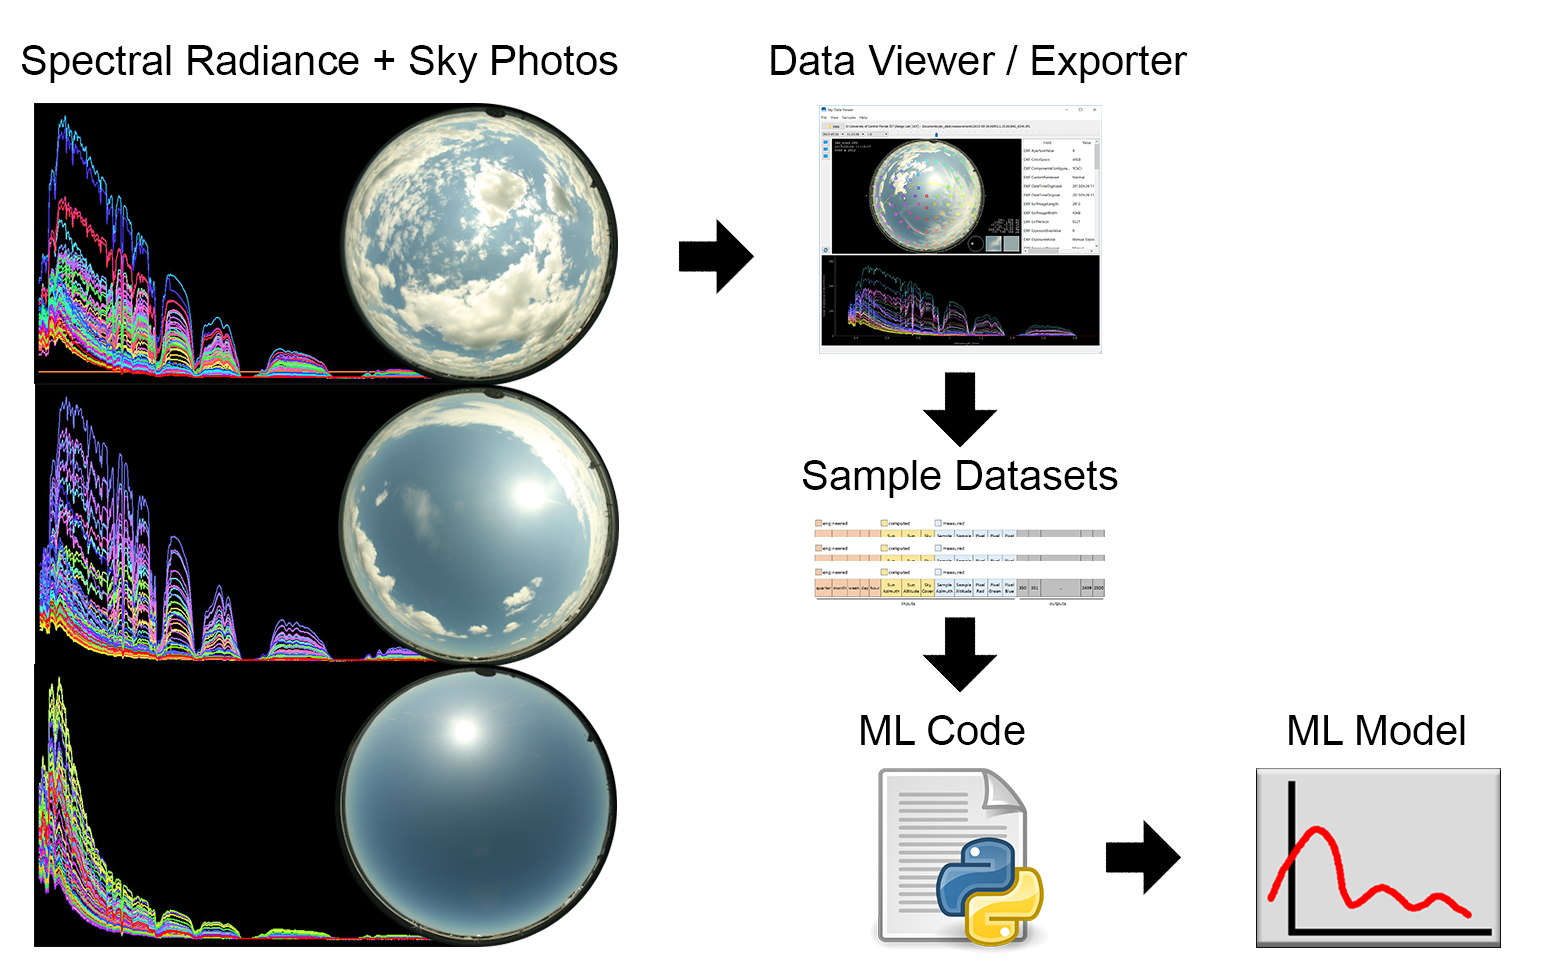
\includegraphics[width=0.448\textwidth]{img/story_train.png}
	& & &
	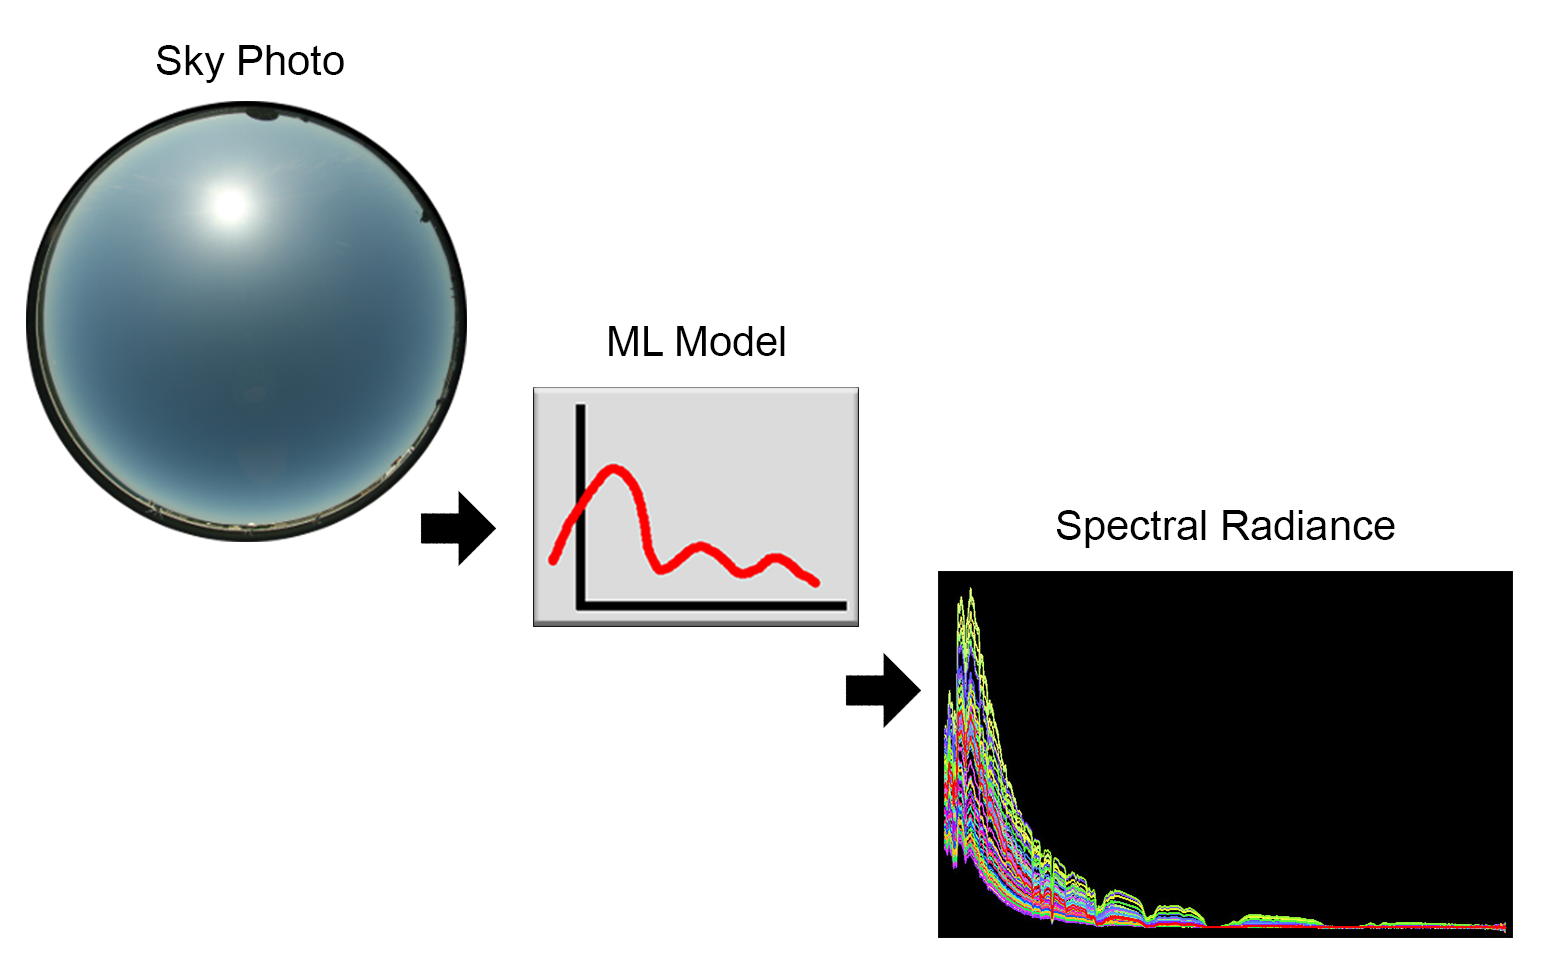
\includegraphics[width=0.448\textwidth]{img/story_predict.png}
	\\\arrayrulecolor{tablegrey}\hline
	\cellcolor{blue!11} \footnotesize {Offline Learning (Precomputation)} &\cellcolor{blue!11} &\cellcolor{red!11} & \cellcolor{red!11}\footnotesize{Whole Sky Spectral Radiance Estimation (Real-time)}
	\\\arrayrulecolor{tablegrey}\hline
\end{tabular}
\end{center}\vspace{-2mm}
\caption{We estimate sky radiance distribution curves between 350-2500nm from images captured with a digital camera. (Left) We use measurements from a commercial digital camera and a sky scanning spectroradiometer to train machine learning algorithms. (Right) We then utilize this ML model to take new sky images and produce the whole sky spectral illumination in real-time.
We have validated this approach to measured data.
}
\label{fig:teaser}
\end{figure}
\vfill

% text
\begin{abstract}
\label{sec:abstract}
This work proposes estimating sky radiance distribution curves between 350-2500nm from images captured with a hemispherical digital camera. A novel hardware system simultaneously captured spectral, spatial, and temporal information to acquire accurate physical measurements of the solar/skydome radiance variation. To achieve this goal, we use a custom-built spectral radiance measurement scanner to measure the directional spectral radiance, a pyranometer to measure the irradiance of the entire hemisphere, and a commercial digital camera to capture high-dynamic range (HDR) hemispherical imagery of the sky. We use the measurements obtained from a commercially available digital camera and correlating spectroradiometer measurements to train machine learning (ML) models to estimate whole sky full-spectrum radiance distributions (VIS, VNIR, and SWIR) from a low dimensional RGB input. We train clear, cloudy, and mixed sky models, and cross-validate the estimated radiance distributions with ground-truth data. We highlight important measured and engineered ML features, and we present useful feature engineering techniques employed to minimize model estimation error. Additional contributions of this work include the code for all ML models and experiments, a dataset of all-sky HDR captures with correlating spectroradiometer measurements captured 453 times over 16 days, and an open-source, cross-platform, interactive viewer used to visualize photometric and radiometric data side by side.
\end{abstract}
\keywords{Sky Radiance, Radiance Distribution, Multispectral, Machine Learning, Regression, Sky Viewer}
\section{INTRODUCTION}
\label{sec:introduction}

Multispectral sky radiance is needed for wavelength dependent computations in a wide variety of domains and applications, including: radiative transfer,\cite{chandrasekhar_radiative} building-performance simulation,\textsuperscript{\citenum{jakica_survey},\citenum{hensen_buildingperformance}} photovoltaic (PV) panel alignment\cite{smith_tilt}, climate science,\cite{lopez-alvarez_using_2008} physically based rendering\textsuperscript{\citenum{jakob_mitsuba},\citenum{haber_physically}} natural light transport,\textsuperscript{\citenum{veach_metropolis},\citenum{jarosz_montecarlo}} and any thermal/lighting application using bidirectional reflectance distribution functions (BRDFs).\cite{kurt_survey, cook_torrance_brdf, deering_atmospheric, nicodemus_brdf} The spectra ranges of interest can vary based on a number of factors; we use the following: visible (VIS) (380-780nm), visible and near-infrared (VNIR) (380-1400nm), and short wave infrared (SWIR) (1000-2500nm). Of even more importance is the need for collections of whole sky angular dependent radiance distribution curves required for accurate computations on surfaces affected by the angle of incidence, e.g. walls, facades, PV panels, all of which require more than just a single downward-welling radiance measurement, and all of which need to account for occlusions of the visible skydome.\cite{schumann_environment} Despite the fact that skylight itself has been studied for well over one hundred years (going back to Lord Rayleigh\cite{strutt_lightfromsky_1871}, Mie\cite{mie_beitrage_1908}, Kimball\cite{kimball_intensity}, and Pokrowski\cite{pokrowski_1929}, to name a few), the process of actively measuring or even computing whole sky radiance distributions quickly and accurately still remains an open problem, especially if the curves are to be used in a real-time, practical setting. Reliable, fast, cost-effective methods are still desired. This work attempts to use various modern machine learning methods to train models with the express purpose of being used in a real-time setting to estimate whole sky radiance curves quickly, within some acceptable error, using a dataset of whole sky images and radiance distributions measured with a custom-built hardware system.\cite{kider_framework_2014}

% \begin{figure}[btp]
% \begin{center}
% \includegraphics[width=1.0\textwidth,height=0.25\textwidth]{img/intro_vns.jpg}
% \end{center}
% \caption{\label{fig:spectrum}Sky radiance distribution spectra of interest: VIS, VNIR, and SWIR.}
% \end{figure}

% Some relevant contributions to this problem in the last decade include the following: Refs. \citenum{saito_estimation_2016, chauvin_modelling_2015, kocifaj_unified_2015, tohsing_validation_2014, cordero_downwelling_2013, roman_calibration_2012, ehrlich_airborne_2012, pissulla_comparison_2009, lopez-alvarez_using_2008, cazorla_using_2008, cazorla_development_2008, lee_jr_measuring_2008, milton_estimating_2006}.

Saito et al. estimated sky radiance distributions with a derived equation taking total ozone column and RAW RGB counts.\cite{saito_estimation_2016} They specifically attempt sky radiance estimation \enquote{without any training sets,}\cite{saito_estimation_2016} but focus on a single point in the sky (the zenith) for a subset of visible wavelengths (430-680nm). An important contribution is their camera-specific color matching functions (CMFs), an extension of work done by Sigernes et al.,\cite{sigernes_sensitivity} which take into account camera lens wavelength dependence, vignetting effect, and CMOS noise.\cite{saito_estimation_2016} 

Tohsing et al. used a machine learning approach to estimate full visible spectrum whole sky radiance distributions. They used non-linear regressions, one per color component (RGB) per wavelength (380-760nm), or 1143 models, using the non-linear relationships between RGB counts and radiance values.\cite{tohsing_validation_2014} Although they use 113 sampled points of the hemisphere, their measurements are limited to 8 of 12 consecutive days of the year, with only 1 day's clear sky data and 1 day's overcast data used for training.\cite{tohsing_validation_2014} They classify sky cover procedurally into 2 groups (clear or cloudy) via sky index,\textsuperscript{\citenum{yamashita_cloud},\citenum{saito_cloud}} and train 2 separate groups of regressions; scattered skies thus use one or the other. Because full hemisphere measurements took 12 minutes to complete, a synchronized, synthetic image was constructed and sampled.

Chauvin et al. also used a custom-built sky viewer/imager to obtain and then remove/clean anisotropy from clear sky portions of sky images for better cloud detection and ultimately better solar plant control.\cite{chauvin_modelling_2015} As stated by the authors, they focus on irradiance/intensity as opposed to radiance curves. Conversely to many sky models, they build upon the work of Grether et al. and Buie et al., noting the importance of the circumsolar region and its ratios along with the central angle from sun position to point position, sun-to-point angle (SPA), and explain how it can be used to estimate clear sky radiance.\cite{chauvin_modelling_2015}

Cazorla, Olmo, L\'{o}pez-\'{A}lvarez, and Alados-Arboledas, et al. used a variety of machine learning techniques, including artificial neural networks (ANN), genetic algorithms (GA) and pseudoinverse linear regression, in a series of projects using images from their own custom-built sky viewer.\cite{lopez-alvarez_using_2008, cazorla_using_2008, cazorla_development_2008} The ANN was used to perform cloud detection using color features extracted from sky images while the GA was used to optimize/minimize these features for the input layer of the network.\cite{cazorla_development_2008} A pseudoinverse linear regression model was used on a datatset of 902 samples of sky image RGB values and visible spectrum radiance at $45\degree$, $60\degree$, and $90\degree$ zenith angles. The final training set is whittled down to 40 samples.\cite{cazorla_development_2008}

Kocifaj's model, while well researched and presented, might be too computationally expensive for a real-time application, and is therefore tangential to this project.\cite{kocifaj_angular_2012, kocifaj_unified_2015} Cordero et al. studied albedo effect on radiance distributions (both upwelling and downwelling).\cite{cordero_downwelling_2013} Lee studied overcast skies to find meridional consistencies.\cite{lee_jr_measuring_2008} Pissulla et al. compare 5 separate spectroradiometers and present their measurement deviations.\cite{pissulla_comparison_2009} %Juan and Da-Ren present 3 (geometric, optical, and radiometric) calibration experiments on a sky viewer/imager.\cite{juan_calibration_2009}

A discussion on sky radiance distributions is not possible without acknowledging turbidity and its attenuating effects on terrestrial solar radiance. Rayleigh,\cite{strutt_lightfromsky_1871} Mie,\cite{wriedt_miereview_2012, wriedt_miebook_2012, mie_beitrage_1908} and non-selective scattering algorithms explain it. Although it must be accounted for in models of highest accuracy, it can sometimes be ignored or roughly estimated. There is a wealth of literature in the atmospheric and solar energy communities that highlight the consistency of the ``cosine factor" of solar zenith angle (SZA) on radiance curves, starting with Steven and Unsworth in the mid-1970s, who recorded standard radiance distributions of clear skies, and in doing so found \enquote{departures due to variation in atmospheric turbidity [...] to be small}.\cite{steven_standard_1977}

% This paper is organized as follows. In Section \ref{sec:datacapture} we explain our data capture hardware (\ref{sec:hardware}), measurements (\ref{sec:measurements}), and observed data (\ref{sec:data}). In Section \ref{sec:methods} we explain our methods and experiments for spectral shape estimation. Results are presented in Section \ref{sec:results} with concluding remarks in Section \ref{sec:conclusions}.
\section{Data Capture}
\label{sec:datacapture}

\subsection{Hardware}
\label{sec:hardware}

We utilized the capture setup proposed by Kider et al. to capture data needed to train and predict sky radiance distribution curves for the sun/skydome\cite{kider_framework_2014}. This novel hardware system captured spectral, spatial, and temporal information, including radiance, HDR fisheye imagery, and total irradiance, simultaneously for various sky conditions. Fig.~\ref{fig:hardwarejtk}(left) shows the capture setup on the roof of a building. The system includes a custom-built spectral radiance measurement scanner to measure the directional spectral radiance, using an ASD FieldSpec Pro spectroradiometer to capture field measures of the solar spectrum between 350-2500nm (Fig.~\ref{fig:hardwarejtk}(a)). The system used a commercial digital camera to capture HDR hemispherical imagery of the sky, using a Canon 5D with a Sigma 8mm circular fish-eye lens, following a similar scanning technique to Stumpfel et al.\cite{Stumpfel:2004}. This approach utilized 8 exposures to span a range of 17 stops of the sun and sky to capture a wide dynamic range (Fig.~\ref{fig:hardwarejtk}(b)). Lastly, the system used an Apogee pyranometer to measure a total irradiance value of the sun/sky (Fig.~\ref{fig:hardwarejtk}(c)).

\begin{figure}[hbtp]
\begin{center}
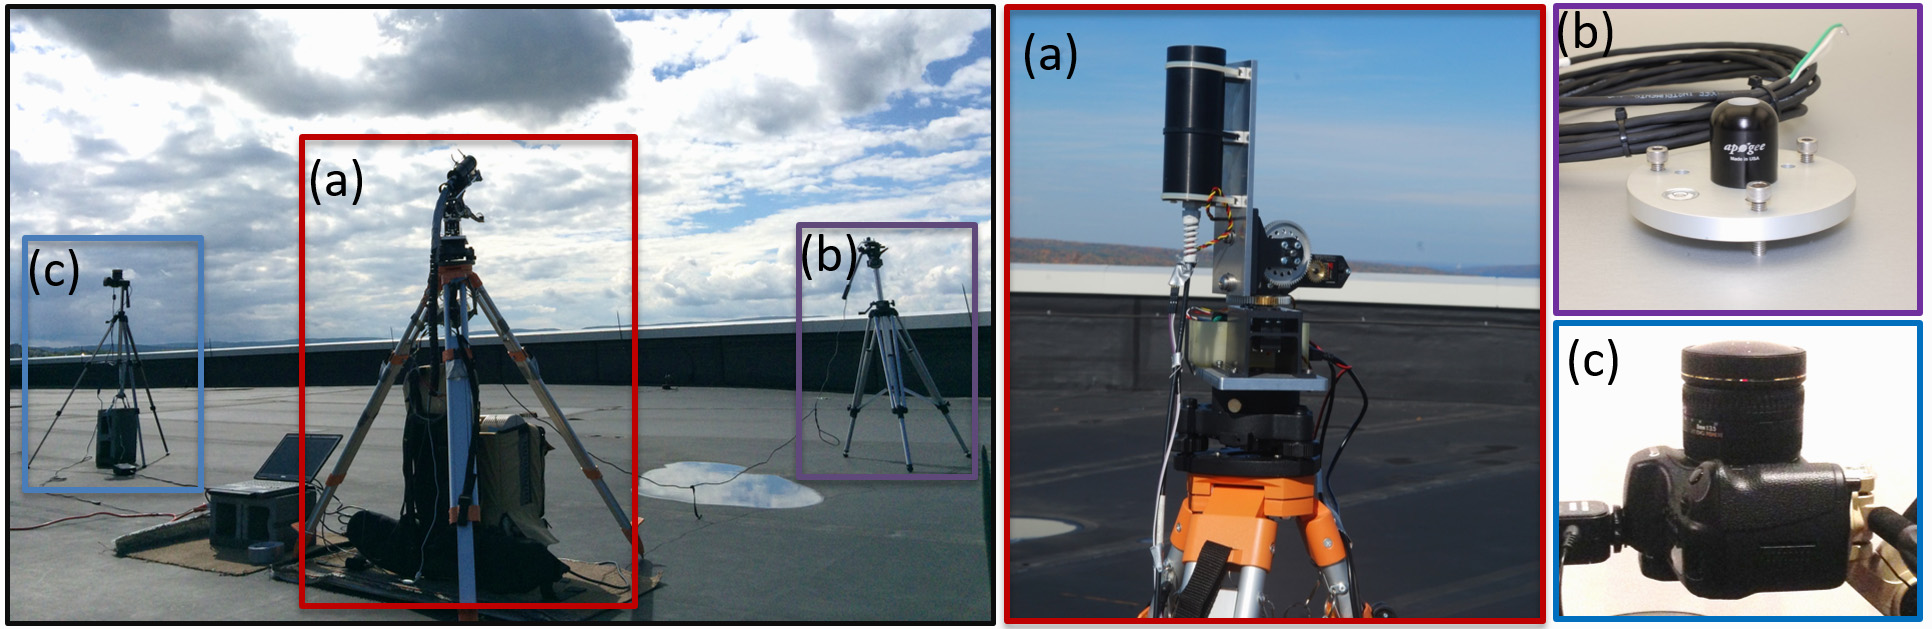
\includegraphics[width=0.98\textwidth]{img/hardware.jpg}
\end{center}\vspace{-2mm}
\caption[hardwarejtk] {\label{fig:hardwarejtk} Hardware setup of different capture devices from Kider et al.\cite{kider_framework_2014} used to capture data for this project. (a) A custom-built radiance scanner measures spectral radiance between 350-2500nm using a $1\degree$ fore-optic lens; (b) Apogee pyranometer, which measures the irradiance of the entire sun/sky; (c) Canon 5D commercial camera with Sigma 8mm circular fish-eye lens captures HDR imagery of the sun and skydome.}
\end{figure}

\subsection{Measurements}
\label{sec:measurements}

\begin{figure}[hbtp]
\begin{center}
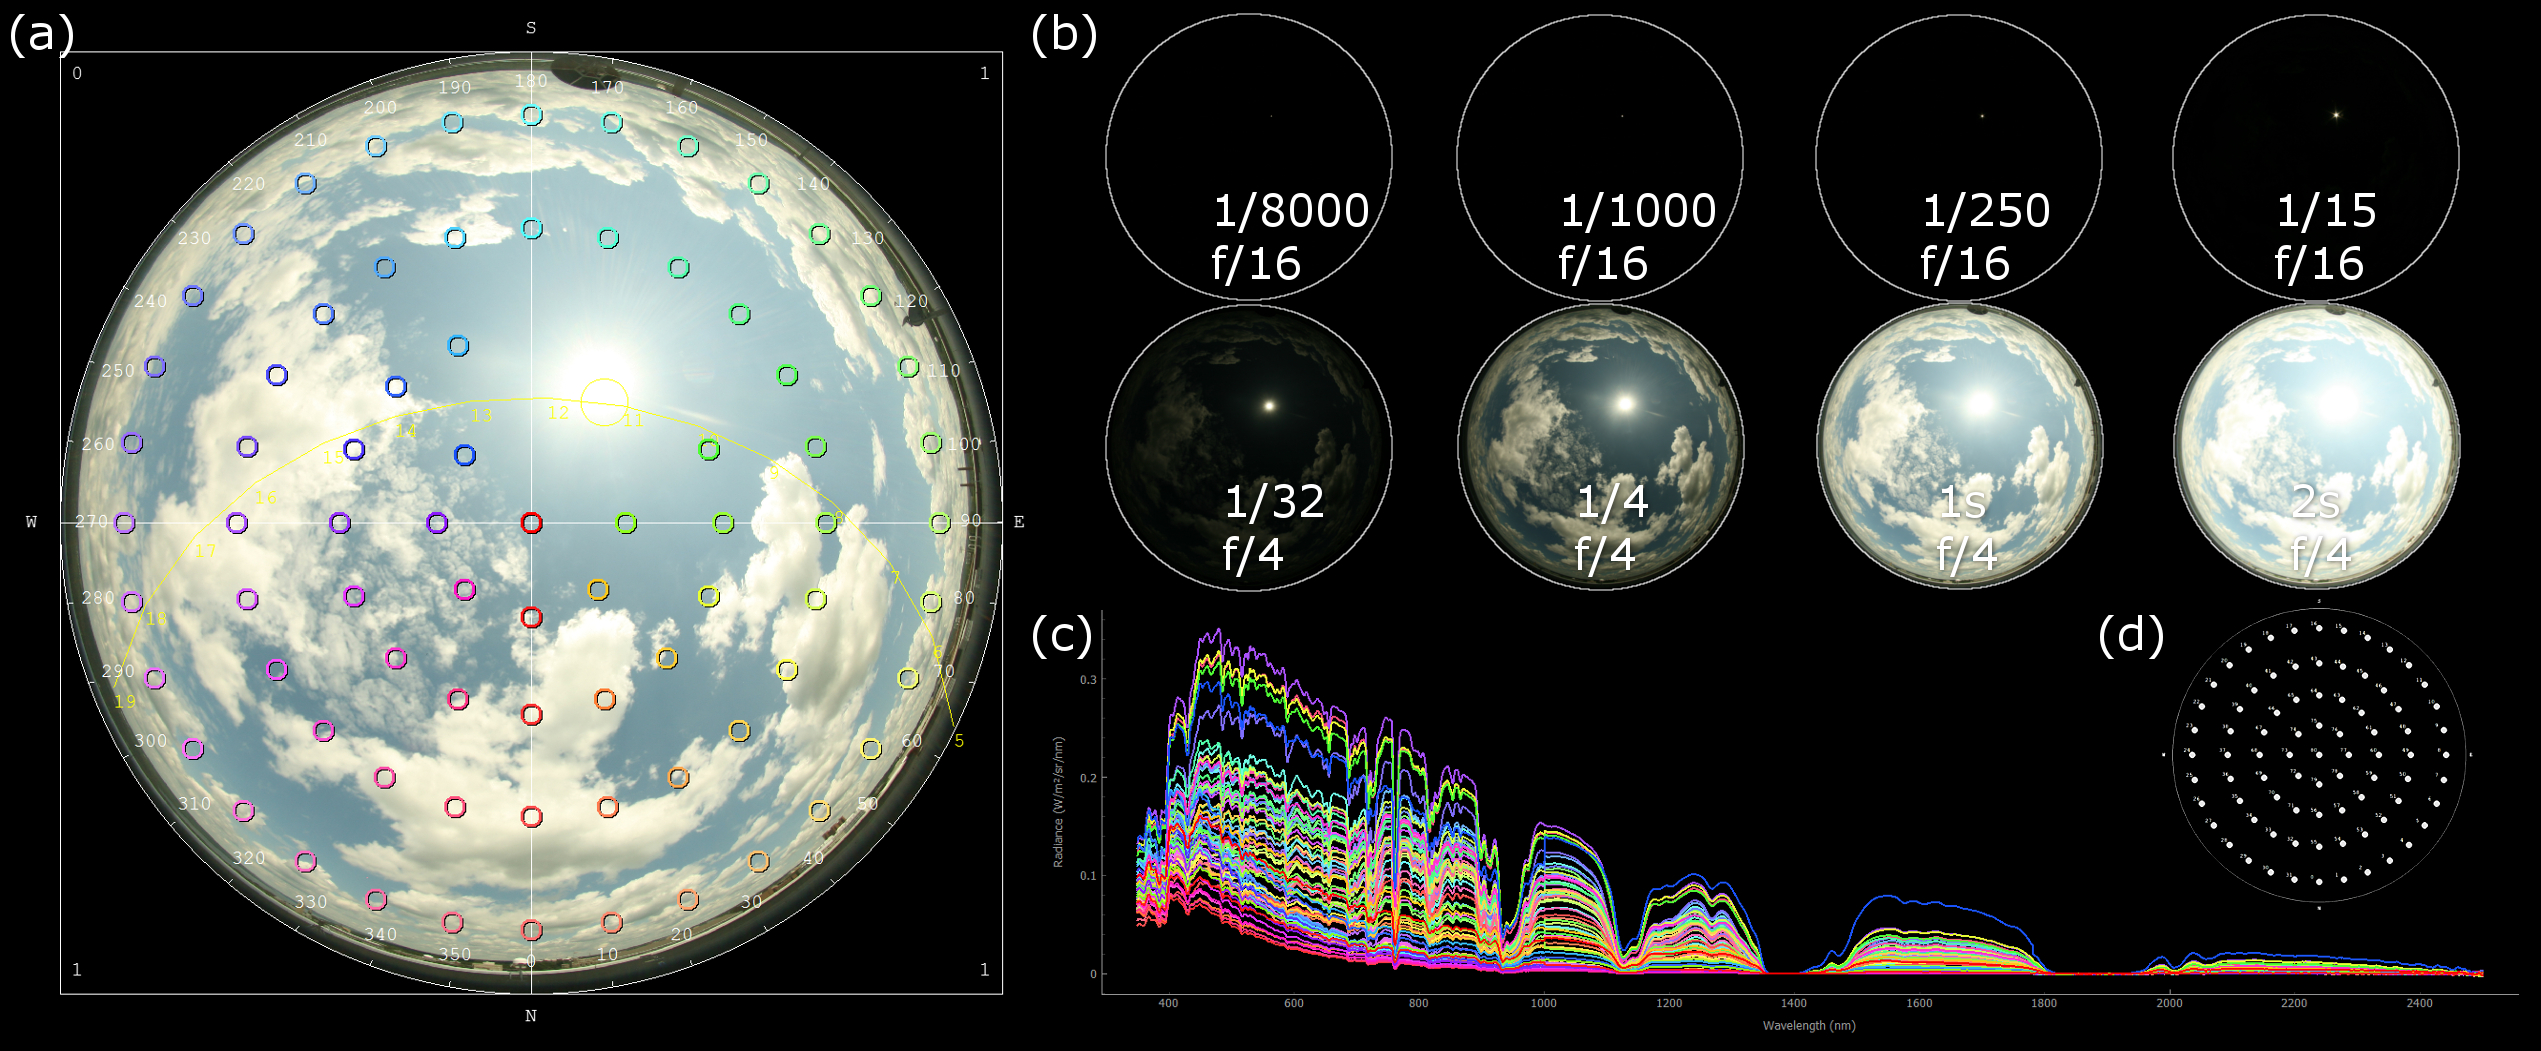
\includegraphics[width=1.0\textwidth]{img/data_measurements.jpg}
\end{center}
\caption{\label{fig:measurements}Each data capture includes: (a) a hemispherical photo of the sky, at (b) 8 separate exposures (HDR), and (c) corresponding sky radiance curves, measured at 81 points in the sky with sampling pattern (d). Applying $20\degree$ circumsolar avoidance, only 76 of the 81 points of measurement are shown in (a).}
\end{figure}

% \begin{figure}[H]
% \begin{minipage}{0.45\linewidth}
% \centering
% \includegraphics[width=1.0\textwidth]{img/data_samples.png}
% \end{minipage}%
% \begin{minipage}{0.53\linewidth}
% \centering
% \includegraphics[width=1.0\textwidth]{img/data_exposures.png} \\
% \includegraphics[width=1.0\textwidth]{img/data_radiance.png}
% \end{minipage}
% \caption{\label{fig:measurements}Each data capture includes: (a) hemispherical photo of the sky, (b) with 8 separate exposures (HDR), and (c) corresponding sky radiance distributions measured at 81 points in concentric rings. Applying $20\degree$ circumsolar avoidance, only 76 of the 81 points of measurement are shown in (a). }
% \end{figure}

% \begin{figure}[H]
% \begin{center}
% \begin{tabular}[b]
% \includegraphics[width=0.4\textwidth]{img/data_samples.png}
% \end{tabular}
% \begin{tabular}[b]
% \includegraphics[width=0.6\textwidth]{img/data_radiance.png} \\
% \includegraphics[width=0.6\textwidth]{img/data_radiance.png}
% \end{tabular}
% \end{center}
% \caption{\label{fig:measurements}Types of data we measured...}
% \end{figure}

Throughout this work, hemispherical sky coordinates are specified as $(azimuth, ~altitude)$, where $altitude$ is the complement of $zenith$ (90\degree - $zenith$), and $azimuth$ is a horizontal angle increasing eastward from north. Note that our sky photos have north and south inverted due to hardware orientation during capture.

Sky photos were captured at a resolution of 4368x2912 pixels in both JPG and CR2 (Canon Raw) formats in an sRGB color space (one of the highest pixel resolutions for custom-built sky viewers to date). As shown in Fig.~\ref{fig:measurements}, 8 separate photos were taken in sequence with exposures $1/8000s$, $1/1000s$, $1/250s$, $1/15s$, $1/32s$, $1/4s$, $1s$, $2s$, and $f$-stops $f/16$ and $f/4$. Radiance was measured in $W/m^2/sr/nm$ for 81 evenly distributed $1\degree$ solid angles across the sky. Our spectroradiometer produced a single uniform curve from 350-2500nm, containing VIS (380-760nm), VNIR (380-1400nm), and SWIR (1000-2500nm) spectra.

We used the National Renewable Energy Laboratory's (NREL) Solar Position Algorithm (SPA)\cite{reda_spa} to accurately compute the sun's hemispherical coordinates and path. Some have claimed NREL's SPA algorithm to be too computationally expensive for real-time applications, recommending the SG2 algorithm instead,\textsuperscript{\citenum{blanc_sg2},\citenum{chauvin_modelling_2015}} but we found it to be fast and reliable.

\subsection{Data}
\label{sec:data}

All data for this work was captured between 2012-2013 from the rooftop of Frank Rhodes Hall, Cornell University, Ithaca, New York, United States, decimal degrees: (42.443441, -76.481638). Although we measured data well over 1000 times over 41 days throughout the year, with multiple projects in mind, our vetted subset for this work consists of 453 captures over 16 days at differing times of day, covering many  different solar angles, all four seasons, and in general a wide variety of atmospheric conditions. These measurements are listed in Table \ref{tab:ourdata}, and hosted online for the public's benefit.\footnote{\url{https://spectralskylight.github.io/RadianceEstimationData}}

As noted in Sec.~\ref{sec:measurements}, each data capture consists of 8 sky photos (of varying exposure) and 81 radiance curves. A single training/testing sample consists of information extracted from one of these sky photos along with its corresponding directional radiance measurement. Of our 453 total captures intended to be used for this work, 22996 of the 36693 $(453\times81)$ samples were finally used for training and cross-validation testing. At least 3000+ samples were culled by circumsolar avoidance to avoid the possibility of oversaturation of direct sunlight on our samples, a common approach in many sky models,\cite{chauvin_modelling_2015} and important for our RGB-to-curve mapping. We used the same $20\degree$ region as Tohsing et al.\cite{tohsing_validation_2014} Note the effects of stray light are drastically reduced at an angle of $20\degree$.\cite{saito_estimation_2016} Many of the remaining samples culled from our final datasets are due in some part to careful examination of the measurements. This was done with an open-source, cross platform application we developed to load and visualize the measurements.\footnote{\url{https://spectralskylight.github.io/SkyDataViewer}} Although a supervised process, it allowed us to quickly navigate the abundance of data to identify dropped, locked, missing, obscured, or oversaturated measurements.

Regarding sky cover, although automatic/procedural assessment is certainly possible,\cite{yamashita_cloud, tohsing_validation_2014, saito_cloud, li_cloud, cazorla_development_2008, arking_cloudcover} we manually assessed our images to ensure accuracy during machine learning. Efficient algorithms can and should be used to automatically assess sky cover during real-time application of this work, for determining which trained model to use. Like Lee,\cite{lee_jr_measuring_2008} we use the standard categorization of sky conditions provided by the US National Oceanic and Atmospheric Administration (NOAA).\cite{noaa_fmh1chpt9_2017} We focus on the following three: clear (CLR), scattered (SCT), and overcast (OVC), where CLR and OVC represent 0 and 8 oktas of cloud cover, respectively.\cite{noaa_fmh1chpt9_2017} In this work, SCT is used to describe skies with any cloud coverage between 1-7 oktas. We ignore the distinction of few (FEW) and broken (BKN) skies to simplify the number of machine learning models that might be used in a practical setting. In theory, our models can be trained on any sky condition.

\begin{figure} [hbtp]
\begin{center}
\begin{tabular}{c}
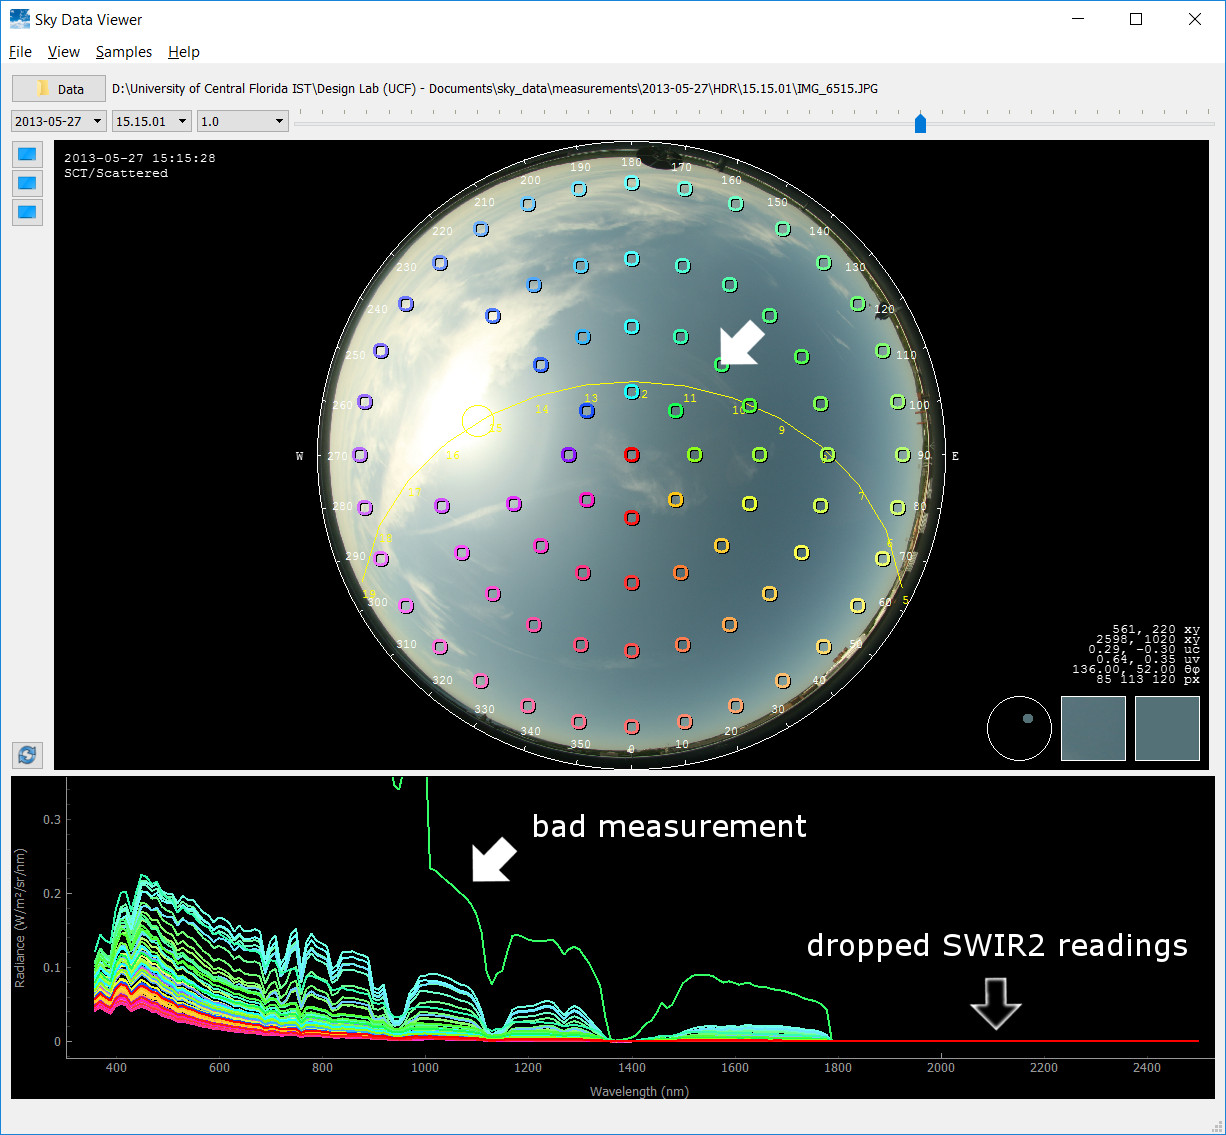
\includegraphics[width=0.485\textwidth]{img/data_badmissing.jpg}
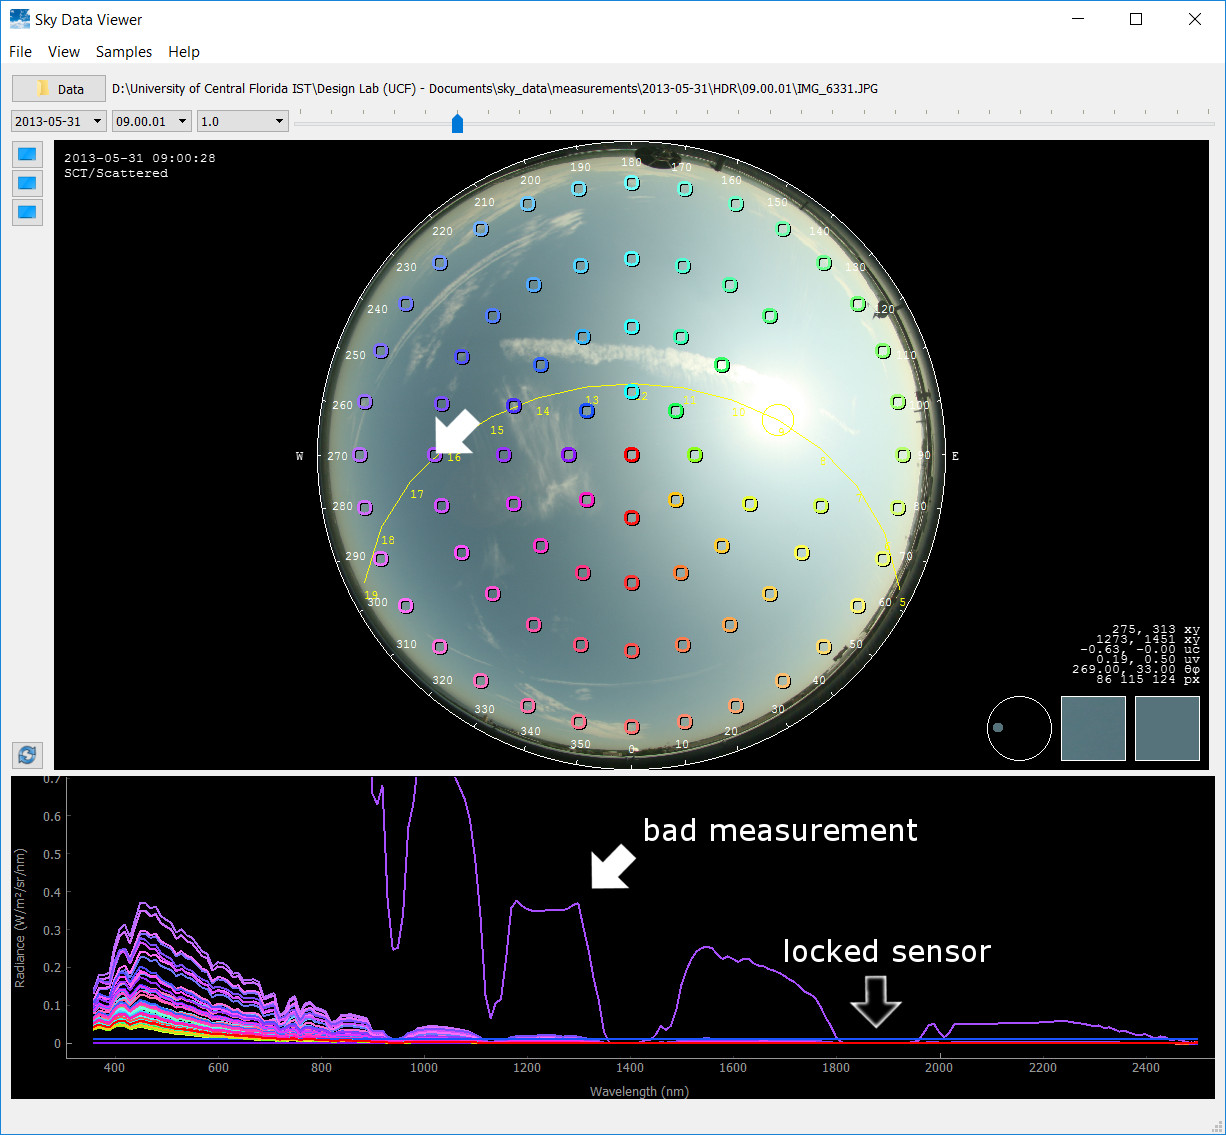
\includegraphics[width=0.485\textwidth]{img/data_badlocked.jpg}
\end{tabular}
\end{center}
\caption[skydataviewer] { \label{fig:skydataviewer} Capturing data \textit{in the wild} for machine learning algorithms is a difficult process. Errors in data capture can vastly affect ML training. Therefore, we developed a SkyDataViewer to help identify data anomalies.}
\end{figure}

\begin{table}[hbtp]
\caption{List of observed data captures, which include correlated HDR images and radiance distributions.}
\label{tab:ourdata}
\centering      
\begin{tabular}{ll*{3}{c}}
    \\
    \toprule
    \multicolumn{1}{c}{Date} & \multicolumn{1}{c}{Time} & Captures & Samples & Sky Cover(s) \\
    \midrule
    \rule[-1ex]{0pt}{3.5ex}  11/06/2012 & 12:26 - 16:21 & 41 & 3321 & SCT  \\
    \rule[-1ex]{0pt}{3.5ex}  11/15/2012 & 11:15 - 16:26 & 56 & 4536 & CLR, SCT  \\
    \rule[-1ex]{0pt}{3.5ex}  04/13/2013 & 09:55 - 10:01 & 2 & 162 & OVC  \\
    \rule[-1ex]{0pt}{3.5ex}  04/14/2013 & 10:42 - 18:36 & 46 & 3726 & SCT, OVC  \\
    \rule[-1ex]{0pt}{3.5ex}  04/15/2013 & 07:38 - 08:03 & 8 & 648 & SCT, OVC  \\
    \rule[-1ex]{0pt}{3.5ex}  05/12/2013 & 10:30 - 13:45 & 14 & 1134 & SCT, OVC  \\
    \rule[-1ex]{0pt}{3.5ex}  05/26/2013 & 10:30 - 17:30 & 29 & 2349 & CLR, SCT  \\
    \rule[-1ex]{0pt}{3.5ex}  05/27/2013 & 09:30 - 18:30 & 37 & 2997 & CLR, SCT  \\
    \rule[-1ex]{0pt}{3.5ex}  05/30/2013 & 09:30 - 12:45 & 14 & 1134 & SCT  \\
    \rule[-1ex]{0pt}{3.5ex}  05/31/2013 & 09:00 - 15:00 & 25 & 2025 & SCT  \\
    \rule[-1ex]{0pt}{3.5ex}  06/15/2013 & 07:45 - 18:30 & 44 & 3564 & CLR, SCT  \\
    \rule[-1ex]{0pt}{3.5ex}  07/26/2013 & 11:00 - 14:45 & 16 & 1296 & CLR, SCT  \\
    \rule[-1ex]{0pt}{3.5ex}  07/29/2013 & 09:00 - 14:00 & 21 & 1701 & SCT, OVC  \\
    \rule[-1ex]{0pt}{3.5ex}  08/30/2013 & 09:15 - 14:00 & 18 & 1458 & SCT, OVC  \\
    \rule[-1ex]{0pt}{3.5ex}  09/24/2013 & 06:49 - 18:09 & 38 & 3078 & CLR  \\
    \rule[-1ex]{0pt}{3.5ex}  09/26/2013 & 08:30 - 15:40 & 44 & 3564 & SCT  \\
    \midrule
    \multicolumn{1}{c}{16 Days} & & 453 & 36693 &  \\
    \bottomrule
\end{tabular}
\end{table}

\section{Spectral Shape Estimation}
\label{sec:methods}

We approached the problem of estimating radiance distribution curves with machine learning (ML), a superset discipline including much of statistics and neural networks. There are a variety of approaches, algorithms, and software frameworks to choose from. For this work, we focused on a small subset, statistical regression models, and used scikit-learn\cite{pedregosa_scikit}, a powerful, popular open source library written in Python and Cython,\cite{behnel_cython} providing most standard ML functionality (supervised/unsupervised algorithms, $k$-fold cross validation, principal component analysis, imputation, etc.).

We use $k$-fold cross-validation (CV), or rotation estimation,\cite{picard_cv,kohavi_cvstudy} to get the most out of our dataset and to minimize the variance of prediction accuracy. We used 10-fold CV specifically to have larger subsamples and less risk of over-fitting. 0 samples from final test captures were used for training, to avoid bias and data leakage.\cite{cawley_overfitting}

In general there are three primary problem categories in machine learning: classification, regression, and clustering, and three primary learning modes: supervised, unsupervised, and reinforcement. Predicting a radiance distribution, essentially a continuous curve of points, using correlated ground truths, is a supervised regression problem. Thus our first task was clear -  we needed to clean, correlate, and export all usable measurements into datasets of input-output mappings (or samples), each of which correspond to a single directional radiance measurement, and each of which would be used for either CV training/testing or final holdout testing. The initial measured (raw) features extracted from our data include: timestamp, pixel colors $(RGB)$, measurement location $(azimuth, altitude)$, and directional radiance values per wavelength. The use of multiple exposure (HDR) pixel values and sky irradiance were left for future/ongoing work, though it stands to reason that multiple pixel values across multiple images can just as easily be used as features, as a single pixel value.

Next, we determined which parameters were needed for our model. Feature engineering, the process of determining which inputs best represent the correlated outputs, is an important and often time-consuming part of any machine learning project.\cite{mitchell_ml, domingos_feature, forman_feature, brownlee_mlmastery} It is not recommended to rely on raw features alone. Too many features may distract an algorithm, while too few may be insufficient to model complex relationships. Investigative exploratory data analysis (EDA) on the raw features gave us insight and preliminary performance metrics, such as the importance of one feature over another, the insignificance of sample azimuth, etc. Fig. \ref{fig:eda} shows a subset of EDA techniques employed.

%I confirm the same results as Brandon's. Replacing drop out data with taking the average of the column and shifting negative values didn't have any impact on regression score.

\begin{figure} [b]
\begin{center}
\begin{tabular}{c}
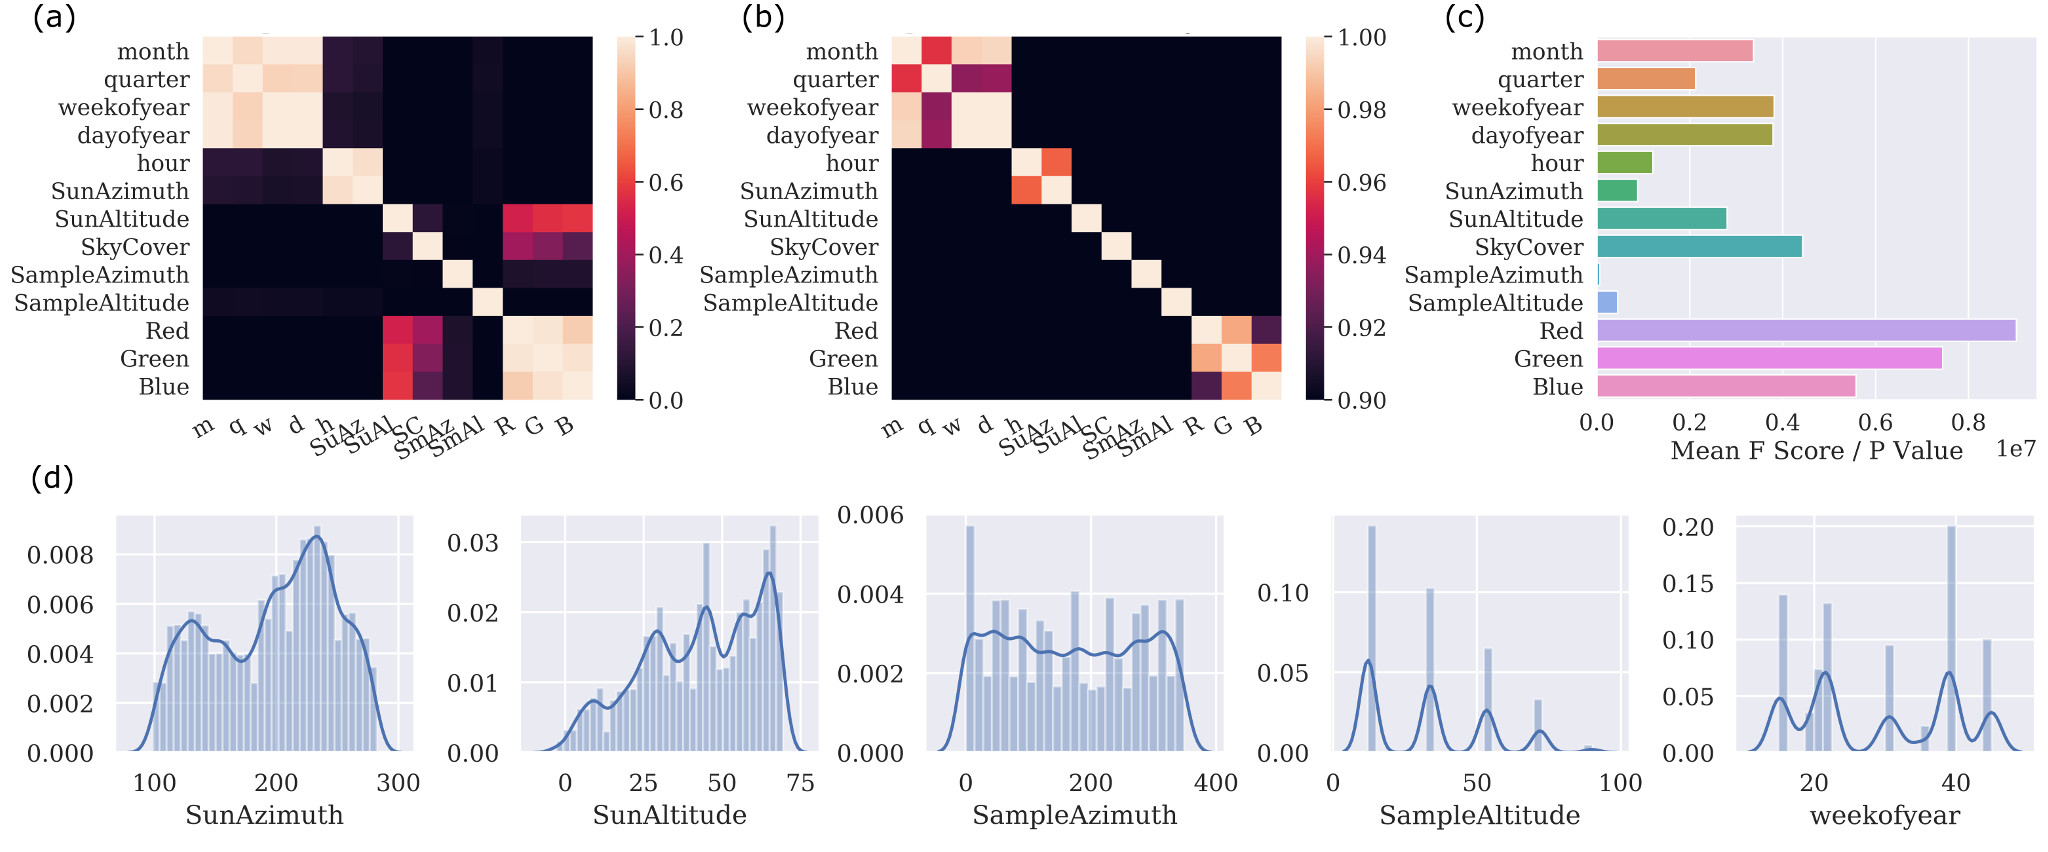
\includegraphics[width=0.98\textwidth]{img/eda.jpg}
\end{tabular}
\end{center}
\caption[eda] { \label{fig:eda}EDA (a) correlation matrix, (b) collinearity matrix, (c) feature importance , and (d) histograms.}
\end{figure}

After EDA, we began searching for an appropriate regression model. Though predicting spectral radiance is clearly a regression problem, it was not so clear which regression model should be used. Many common statistical models (for both regression and classification problems) produce a single output, and thus have high-dimensional input and low-dimensional (i.e. 1) output. We had the exact opposite problem - a handful of input features to predict 2151 values (wavelengths 350-2500nm). Multi-output regression models seemed best suited to the challenge. We started with the simplest possible model as a baseline, the linear regression model (with multi-output support). We refer to this model as LNR. As expected, initial scores were low (since outputs are highly noisy curves, not linear trends), implying under-fitting and the need for more complexity to the inputs.

We accomplished this several ways: (1) by ``binning" the capture timestamp into discretized buckets (quarter, month, week, hour, etc.), (2) by computing the sun's azimuth and zenith/altitude per capture, (3) by tagging samples with sky cover assessment, and (4,5) with polynomial modeling and feature scaling, respectively. In addition to providing a more complex input, method (1) has the benefit of potentially capturing seasonal and daily shifts such as dawn/day/dusk/night, as well as rainy versus arid seasons, all of which have different skies and sometimes trending turbidity.\cite{power_seasonal} Method (2) complies with the motivation for this work, that the sun's zenith/altitude might have a large impact on the shape of a radiance curve. The feature importance graph in Fig.~\ref{fig:eda} confirms this. Summarized by Chauvin et al., when considering radiance at any given point in the sky, of capital importance is the point-to-zenith angle (PZA), the sun-to-zenith angle (SZA), and the central sun-to-point angle (SPA) between them.\cite{chauvin_modelling_2015} We believe the importance of this information is captured by both the measured sample position and computed sun position included in each sample. As mentioned in Sec.~\ref{sec:data}, we used NREL's SPA algorithm for computing sun position per capture.\cite{reda_spa} Method (3) is also discussed in Sec.~\ref{sec:data}. Method (4), polynomial modeling, has been used for decades for problems such as curve fitting.\cite{deboor_splines} We used it to generate a polynomial combination of features from our specified set of inputs along with a polynomial degree (e.g. the set $[a, b]$ becomes $[1, a, b, a^2, ab, b^2]$ with a degree of 2).\cite{pedregosa_scikit} Specifically, we found that using this polynomial modeling technique with a degree of 4 on the inputs of the LNR model, boosted its CV test score considerably. Our final feature engineering contribution, method (5), involved the use of scalers on the inputs: standard, robust, and quantile transformer,\cite{pedregosa_scikit} all of which attempt to spread the input over a uniform distribution and reduce the impact of marginal outliers.\cite{pedregosa_scikit} The quantile transformer in particular had the greatest positive impact, and so we applied, saved, and loaded it alongside our models. After data processing and feature engineering, a final train/test sample consists of the input and output features shown in Fig.~\ref{fig:features}. Future work will include more input features.

\begin{figure} [b]
\begin{center}
\begin{tabular}{c}
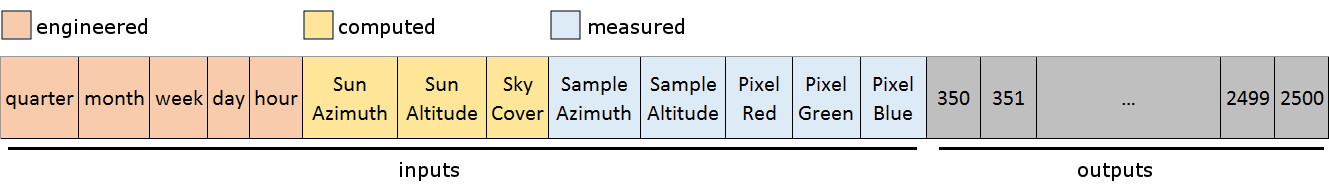
\includegraphics[width=0.98\textwidth]{img/features.jpg}
\end{tabular}
\end{center}
\caption[features] {\label{fig:features}A dataset sample consists of 13 input features and 2151 output features (the radiance curve).}
\end{figure}

We used the following error metrics to compare models and assess prediction performance: coefficient of determination score (R$^2$) and root mean squared deviation (RMSD). We also considered mean bias deviation (MBD), but found it to be ``noisy" without much correlation to R$^2$ and RMSD. We believe this error metric is best suited to a single wavelength, not deviation across a whole curve. The R$^2$ score we used comes from scikit-learn,\cite{pedregosa_scikit} and is defined as:
\begin{equation}
\label{eq:r2}
R^2(x,y) = 1 - \frac{\sum_{i=1}^{N} (x_i-y_i)^2} {\sum_{i=1}^{N} (x_i-\bar{x}_i)^2} ~~\textrm{,}
\end{equation}
where $(x,y)$ is a (truth, prediction) pair, $N$ the number of curves considered, and $\bar{x} = \frac{1}{N}\sum_{i=1}^{N} x_i$~. Note that this score can be negative, despite the name R$^2$. As with Tohsing et al.\cite{tohsing_validation_2014} and others, we used the RMSD metric provided by Iqbal,\cite{iqbal_intro} which indicates the variation of predicted from measured, and is defined as:
\begin{equation}
\label{eq:mbd}
RMSD=\sqrt[]{\frac{\sum_{i=1}^{N} (y_i-x_i)^2}{N}}
\end{equation}
where $N$ is the number of curves considered, $x$ the measured/truth curves, and $y$ the predicted.

\subsection{Machine Learning Models}

After feature engineering and preliminary tests with our polynomial-input linear regression model (LNR), we investigated other multi-output regression models, such as Lasso,\cite{tibshirani_lasso} Ridge,\cite{hoerl_ridge} ElasticNet,\cite{zou_elastic} and Lars. The Lasso linear estimator model has a built-in regularizer, which removes outlier features with low correlation to the output, in an attempt to reduce over-fitting. Ridge is similar, except instead of removing the outliers, it artificially penalizes them to reduce their effect. ElasticNet seems to be a combination of the two. Lars is similar to stepwise regression, in that it finds the most correlated predictors. Though it is typically effective with high dimensional data, it is also sensitive to noise. Unfortunately, as it turned out, all of these models performed no better than LNR, our initial polynomial-input linear regression model, perhaps due to the highly noisy nature of radiance curves, or the fact that we were not over-fitting the data.

The $k$-NN regressor (k-nearest-neighbors or k-neighbors) (KNR) model first gathers all data and then derives predictions from local interpolation of the $k$-closest data points. KNR uses a spatial partitioning tree to organize the data for fast searching and filtering of data points. KNR was the first model we found that performed better than LNR. 

The final model(s) experimented with that performed well were decision tree regressors. Decision tree regression models approximate curves by employing a set of ``if-then-else" rules to predict. The tree depth hyperparameter determines how many rules are used in the tree. If a decision tree regressor becomes too deep, the regressor essentially overfits the data, as the deep chain of rules cannot generalize well. The random forest regressor (RFR)\cite{kocev_tree} and extra tree regressor (ETR)\cite{geurts_etr} both address over-fitting with many separate internal trees for different portions of the dataset, and since each tree is limited in scope, it is not able to overfit. Once final models were chosen, additional hyperparameter tuning was done. Parameters of an ML model are often determined procedurally during training, such as weights and coefficients, whereas hyperparameters are typically specified by the user, such as tree depth or number of trees, etc.

\begin{figure} [hbtp]
\begin{center}
\begin{tabular}{c}
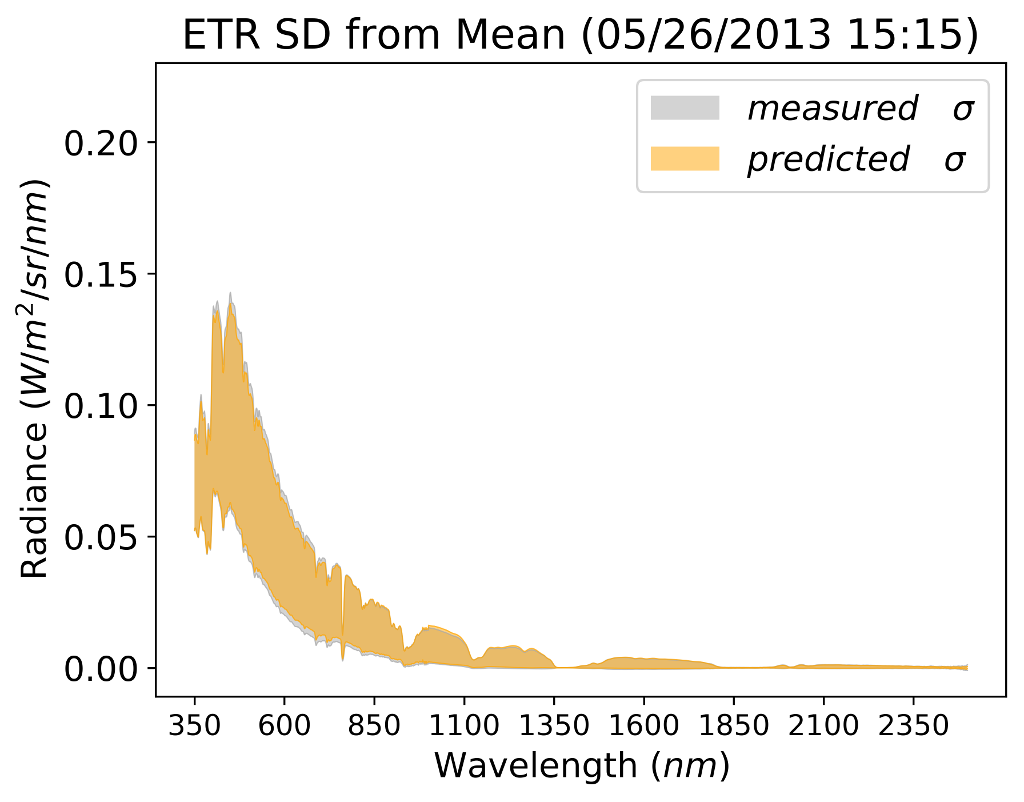
\includegraphics[width=0.32\textwidth]{img/model_etr_sd.png}
%\includegraphics[width=0.32\textwidth]{img/model_rfr_sd.png}
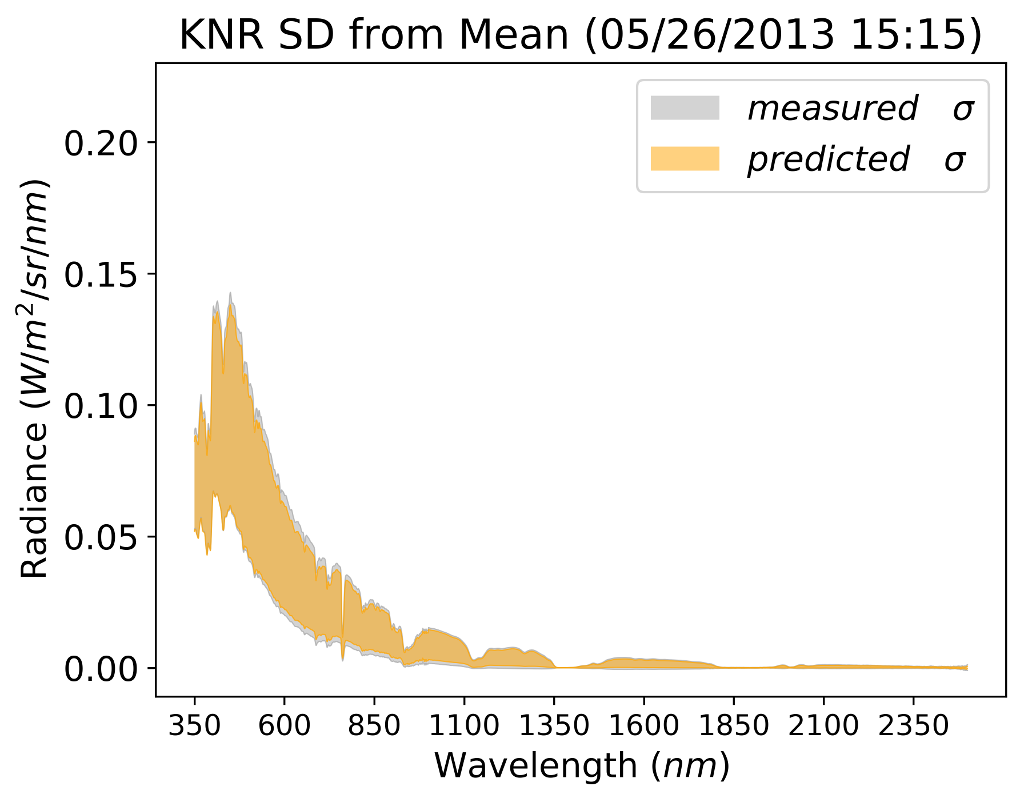
\includegraphics[width=0.32\textwidth]{img/model_knr_sd.png}
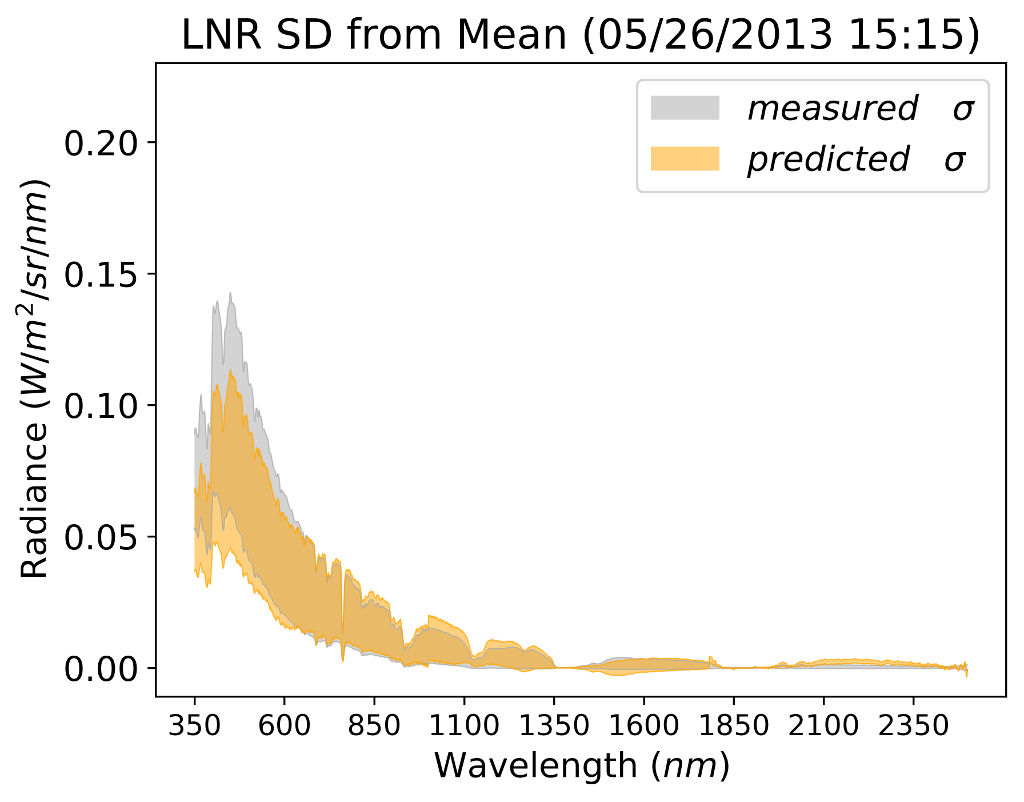
\includegraphics[width=0.32\textwidth]{img/model_lnr_sd.png}
\end{tabular}
\end{center}
\caption[prelimresults] { \label{fig:prelimresults}Three of the four final regression models, ETR, KNR, and LNR, respectively, showing measured and predicted standard deviation from mean on test capture 05/26/2013 15:15 (clear sky). RFR performed very similar to ETR.}
\end{figure}

\begin{table}[hbtp]
\caption[holdout]{Holdout error for final regression models using 10-fold cross validation training and testing over \textit{all usable test samples, across all skies} with train-test ratio of 3:1.\protect\footnotemark}
\label{tab:modelerror}
\centering      
\begin{tabular}{cl*{4}{c}}
    \\
    \toprule
    ID & \multicolumn{1}{c}{Name} & $\mathrm{R}^2$ & RMSD\\
    \midrule
    \rule[-1ex]{0pt}{3.5ex}  ETR & Extra Trees Regressor & 66.55\% & 82.62\% \\
    \rule[-1ex]{0pt}{3.5ex}  RFR & Random Forest Regressor & 62.84\% & 87.09\% \\
    \rule[-1ex]{0pt}{3.5ex}  KNR & K Neighbors Regressor & 58.57\% & 91.95\% \\
    \rule[-1ex]{0pt}{3.5ex}  LNR & Linear Regressor & 51.02\% & 99.99\% \\
    \bottomrule
\end{tabular}
\end{table}

\footnotetext{The high error was mostly due to scattered sky cover predictions, as shown in Sec. \ref{sec:results}}

\subsection{Sky Cover Models}
\label{sec:skycover}

After cross-validated training and testing of our conglomerate (``mix") dataset, with all usable training samples across all sky covers, we suspected that models trained on sky specific datasets might prove more effective. The feature importance graph in Fig.~\ref{fig:eda} confirms this. Thus we filtered the mix dataset into 3 additional datasets (clear, scattered, overcast) based on sky cover assessment (CLR, SCT, OVC, respectively), and divided each of them for CV training/testing and holdout validation testing with our final regression models. The mix dataset contained all usable samples and was almost 1GB in size. Training and testing on a smaller, more focused dataset should be computationally cheaper and possibly even more precise, since the training data better reflects the expected real-world data. As discussed in Sec. \ref{sec:data}, there are a variety of automated/procedural sky cover algorithms that could be employed in a real-time system to assess the input sky images to quickly determine which trained model to use for prediction.  One problem with this experiment was that clear, scattered, and overcast datasets contained 5548, 15508, and 1940 samples respectively (i.e. 24\%, 67\%, and 8\% of total usable samples), and thus overcast skies were not well represented.


\section{Results And Discussion}
\label{sec:results}

\subsection{Regression Models}
\label{result_models}

As the results in Fig. \ref{fig:error_mix} show, when models are trained on all training data across all skies, ETR generally outperforms the rest, with RFR and KNR trading places depending upon the capture. More tests are necessary, but one strategy for real-time application of this work might be triple-mode redundancy,\cite{anderson_tmr} or ``democractic computing," using multiple regressors to predict with (since they are computationally efficient), and using the predicted curves from a specific model based on some decision factor (e.g. standard deviation from mean, etc.)

Although the LNR model was by far the worst performing, we suspect it performed better than expected on some captures (clear skies, possibly with low turbidity) because of the generally similar shape to radiance distributions. As seen in plots showing all measured radiance distributions across a clear sky, as well as time-series plots, the shape of radiance curves can be relatively consistent, often times varying only in magnitude. In this way, each of the coefficients of the polynomial-input LNR model might actually be near-linear as the magnitude of the curve changes. In fact, as Fig. \ref{fig:error_skies} shows, LNR might be usable as-is on some captures (again, as one of several models in a collection of predictors).

\begin{figure} [hbtp]
\begin{center}
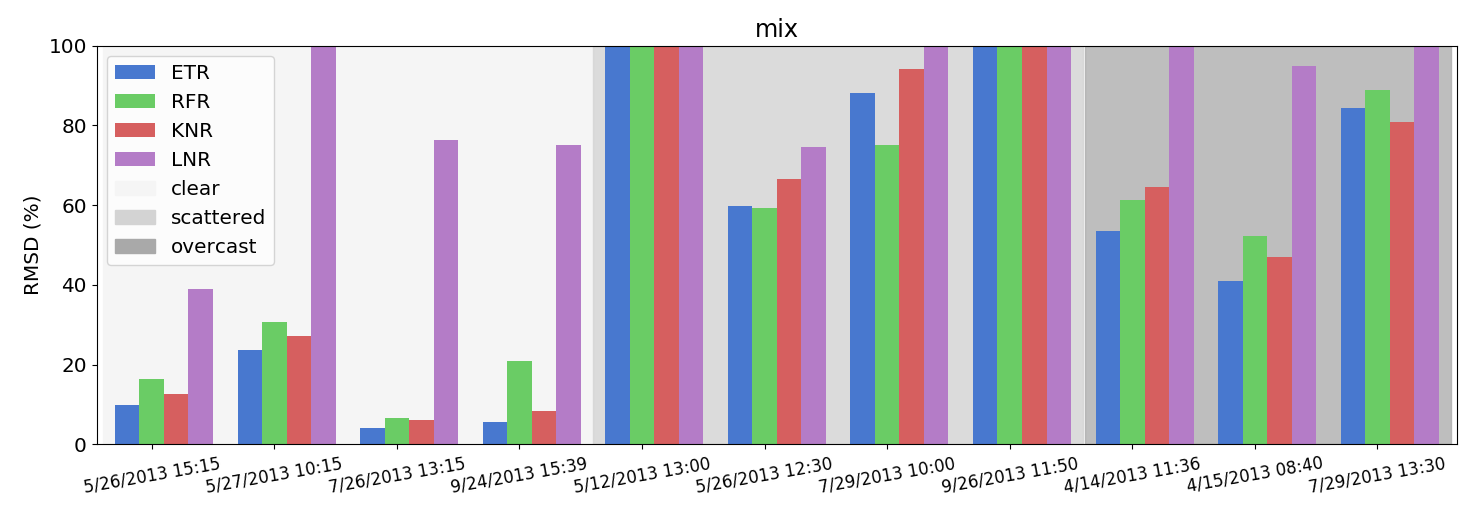
\includegraphics[width=1.0\textwidth]{img/results_mix.png}
\end{center}
\caption[error_mix] { \label{fig:error_mix}RMSD of the models trained with mix dataset, which includes all usable testing samples across all skies.}
\end{figure}

\subsection{Sky Cover}

Final results show that sky cover was extremely relevant, as initially suspected. Three of the four final models were very successful in predicting clear sky captures, shown in Tbls. \ref{tab:resultsETRclear} and \ref{tab:selectcurveerrors}, and Figs. \ref{fig:errorcurves}, \ref{fig:selectcurveratios}, and \ref{fig:wholesky}. LNR even predicted well on two clear sky captures, as mentioned in Sec. \ref{result_models}.

For scattered sky models, RFR's predictions are a surprising success (discussed below). All other models had a hard time with the data. In general, we posit that scattered skies are not predicted well by our methods (as of yet), despite the very large training set of scattered samples. There are a number of reasons why this could be. First, although lens distortions from curvature, vignetting, and even wavelength-specific variation were known to us from Saito et al.,\cite{saito_estimation_2016} we hadn't yet compensated for it in this work. Even a slight shift in sampling coordinates could severely alter the RGB values extracted from the sky images. With clear sky data, that may not be very noticeable, as the color of the sky is fairly uniform, but scattered sky clouds can vary considerably. Future work should definitely compensate for it. Second, the pixel region and weighting algorithms we used may not have been optimal for cloudy skies. Again, clear skies exhibit relatively uniform color whereas clouds and cloud/sky borders can vary, which would distort a final pixel value if weighted over a large enough kernel.

Only three overcast skies were held out for validation, and as mentioned in Sec. \ref{sec:skycover}, only 8\% of the mix dataset were overcast skies (1940 samples). So the results of this experiment on overcast skies are of low confidence. Despite that, ETR, KNR and RFR models were still able to predict one of those three captures with ~40\% RMSD. Given more data, our methods may prove successful on overcast skies as well.

Of particular interest is RFR's performance trained with a mix dataset versus a sky cover specific dataset. RFR performed worse than ETR and KNR on most validation captures when trained with mix. However, it performed equivalent or better than KNR and ETR when trained with sky cover specific data. In fact, as Fig. \ref{fig:error_skies} shows, RFR even predicted scattered skies with semi-acceptable error, something none of the other models were able to accomplish.

\begin{figure} [hbtp]
\begin{center}
\begin{tabular}{c}
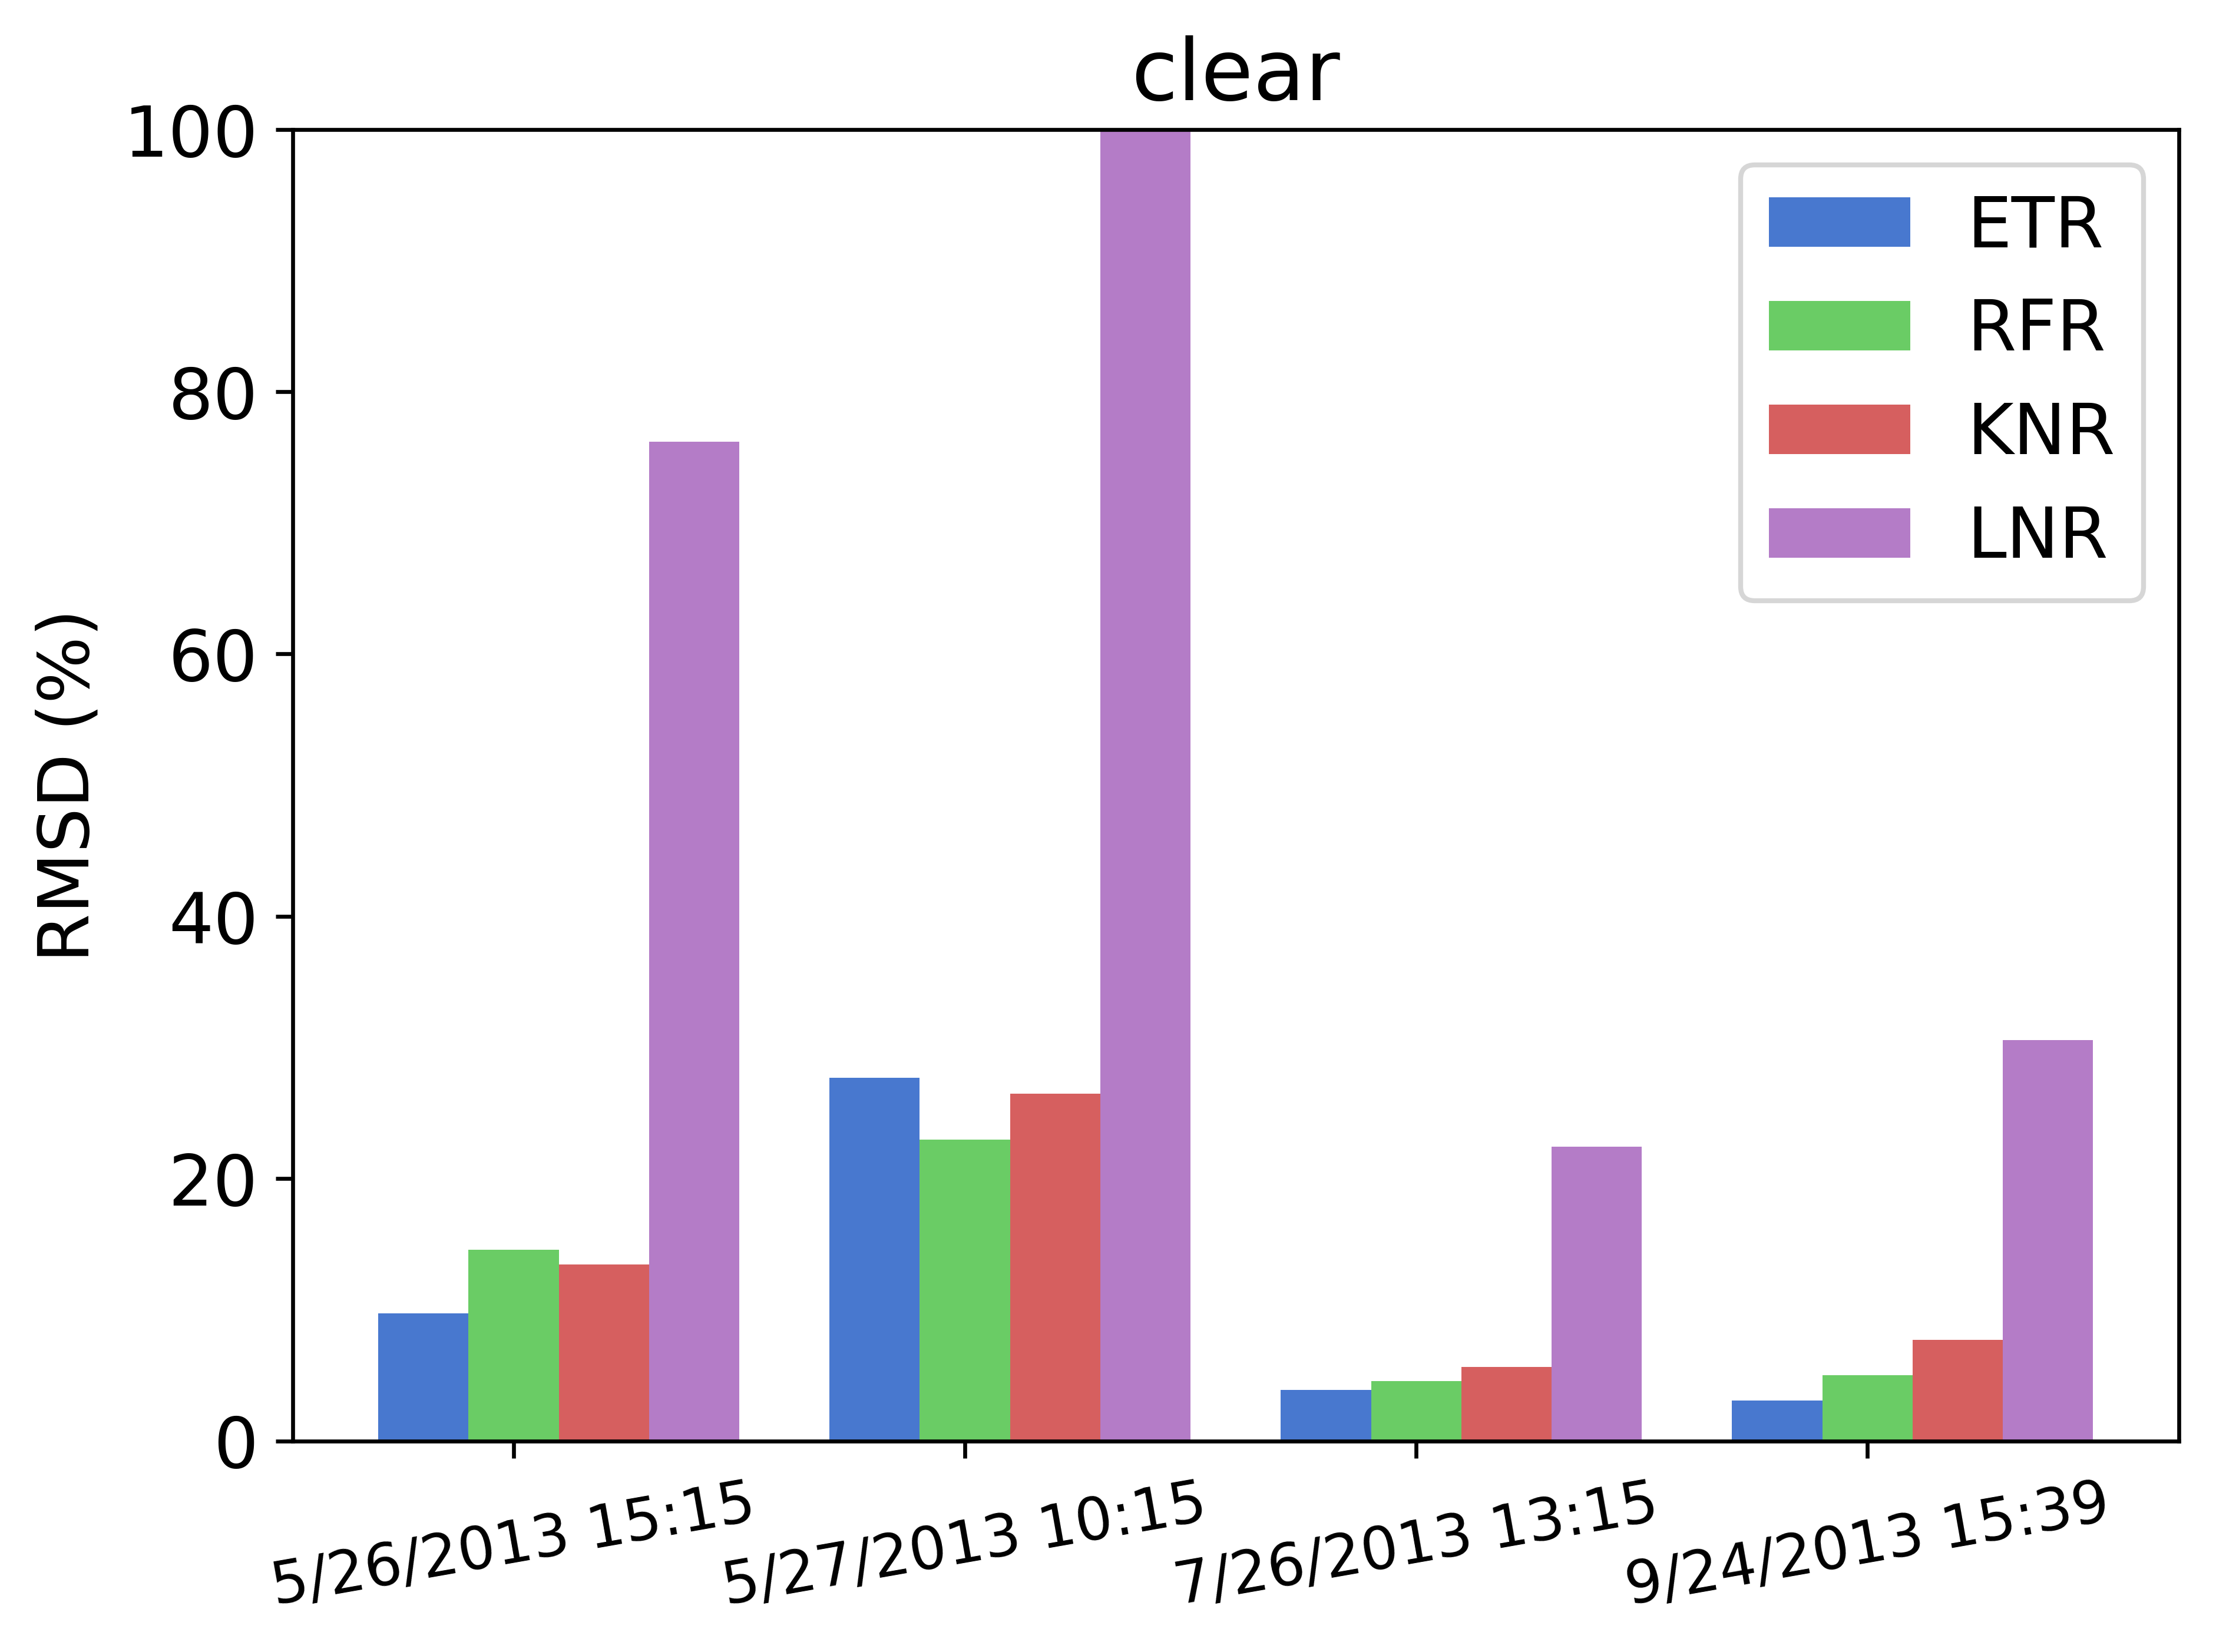
\includegraphics[width=0.32\textwidth]{img/results_clear.png}
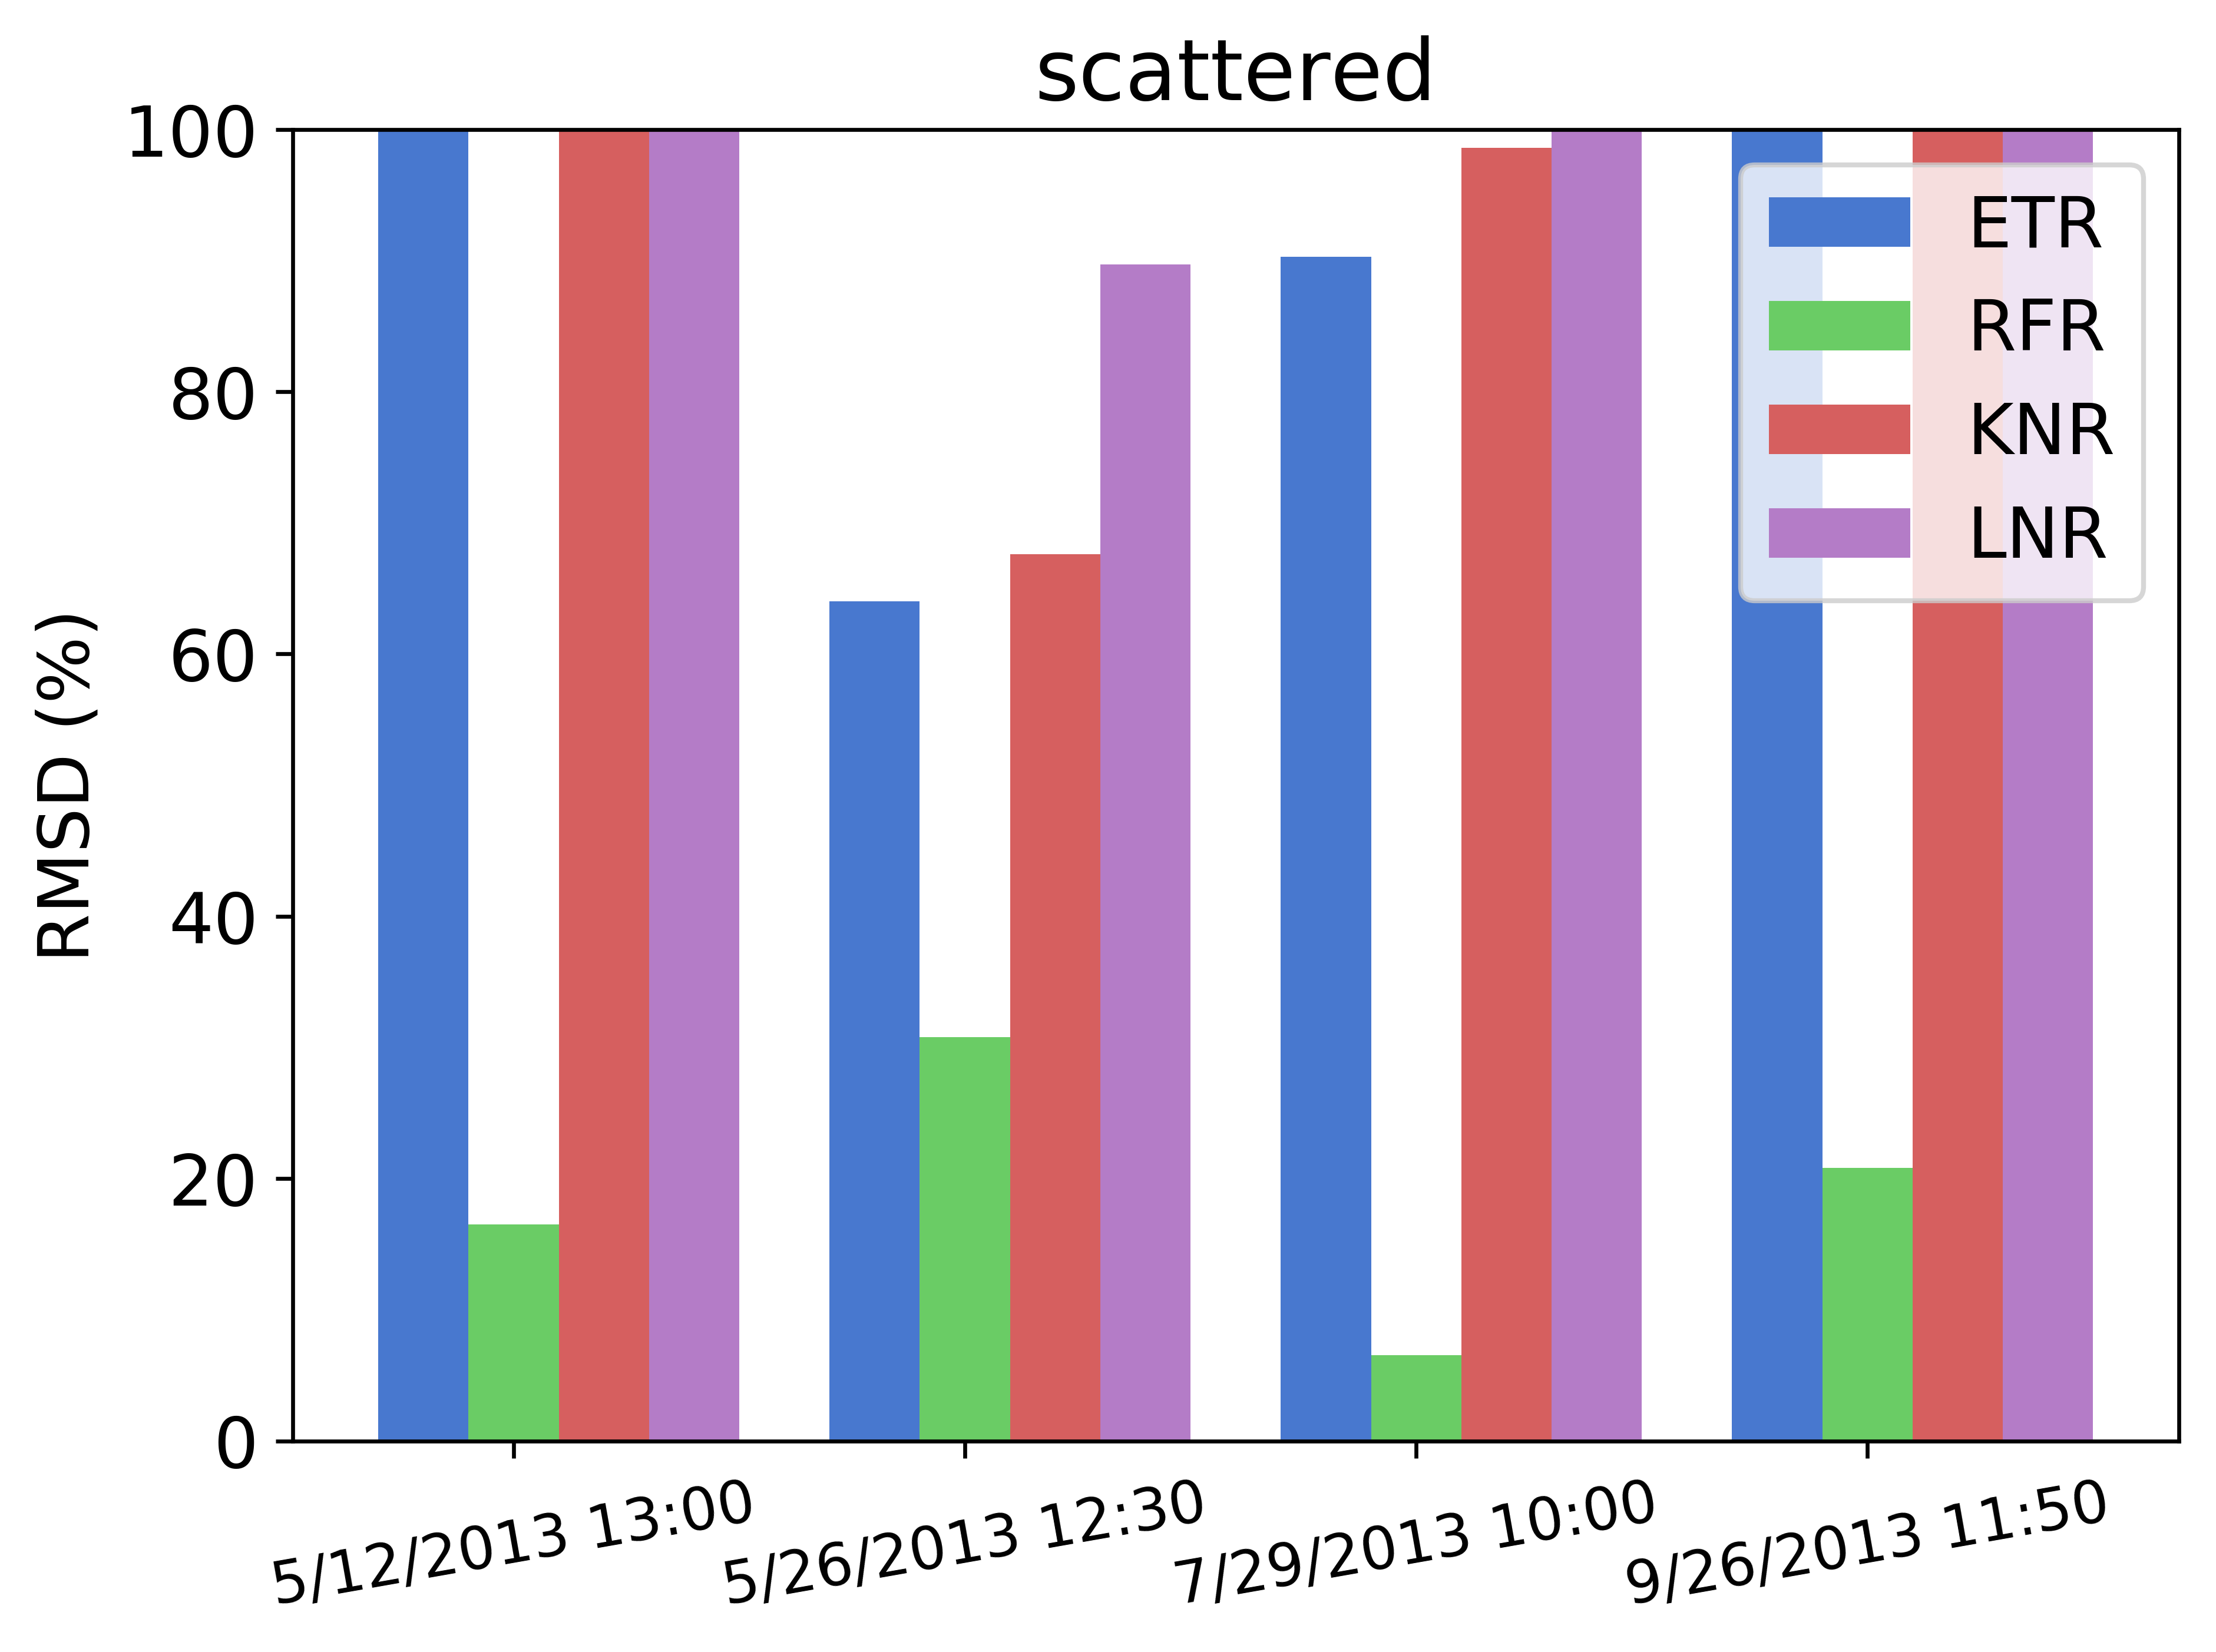
\includegraphics[width=0.32\textwidth]{img/results_scattered.png}
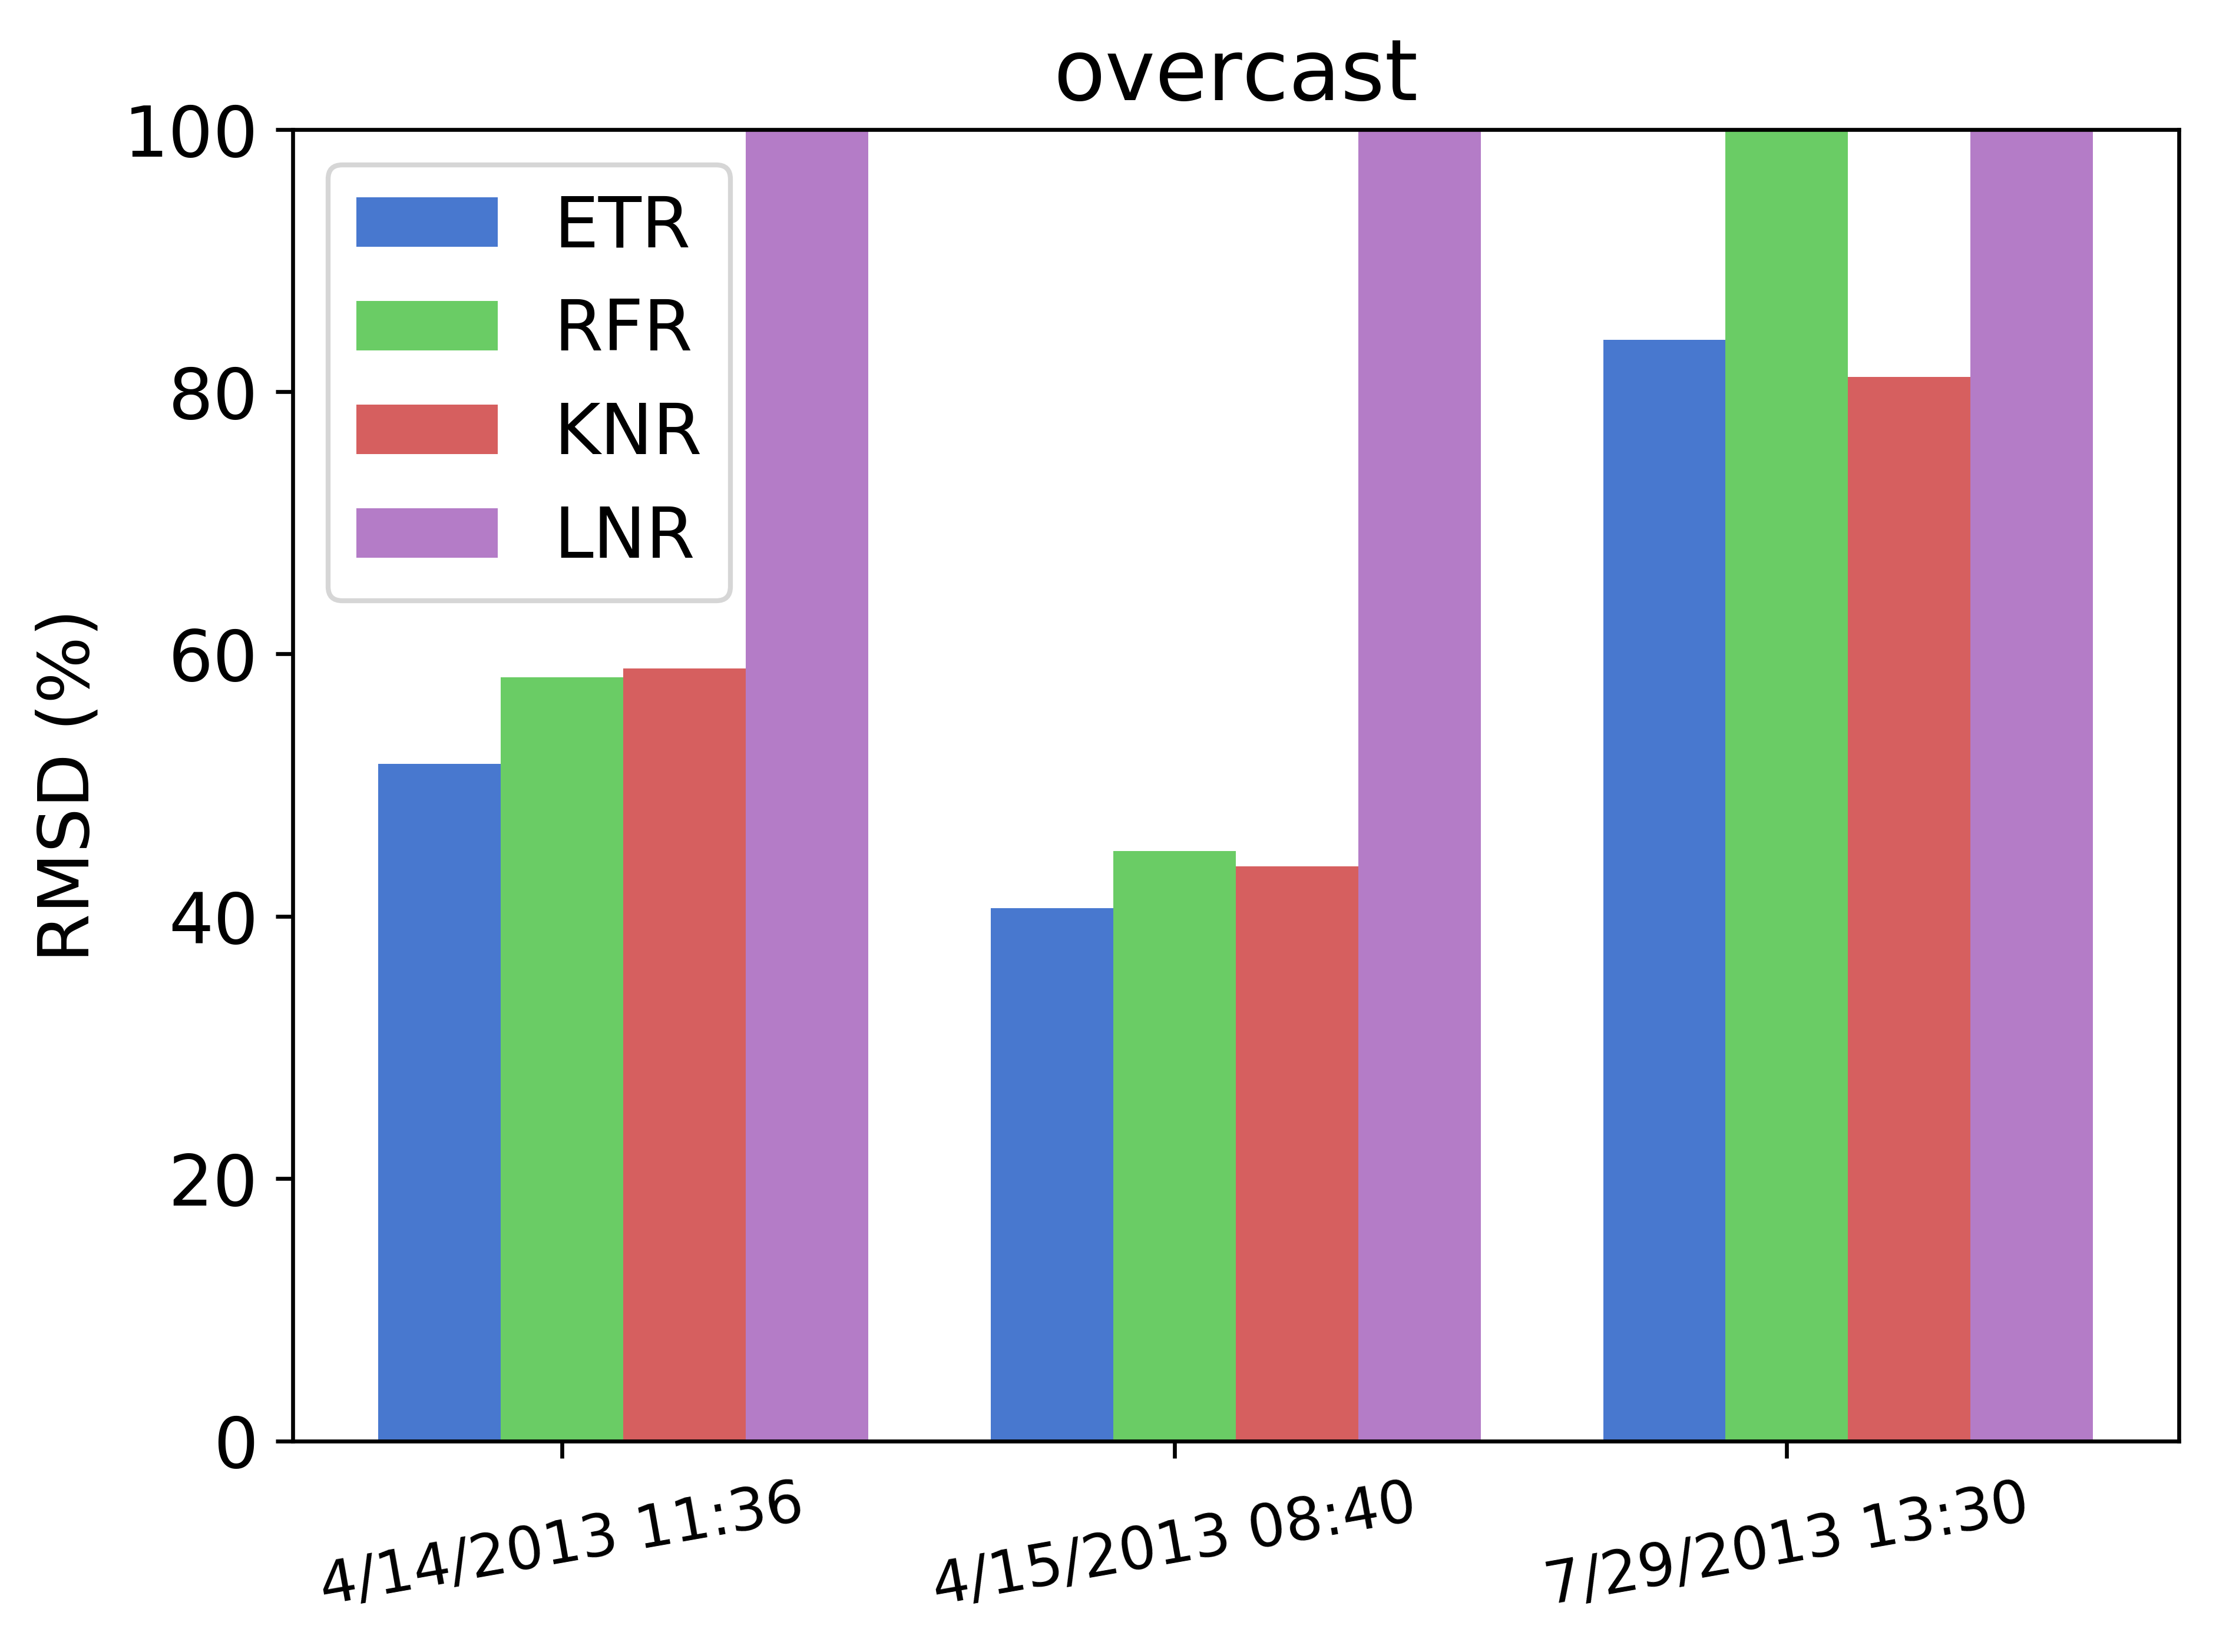
\includegraphics[width=0.32\textwidth]{img/results_overcast.png}
\end{tabular}
\end{center}
\caption[error_skies] { \label{fig:error_skies}RMSD of the models trained with sky cover specific datasets.}
\end{figure}

\begin{table}[hbtp]
\caption{Error metrics for final validation clear sky captures predicted with ETR model clear dataset.}
\label{tab:resultsETRclear}
\centering      
\begin{tabular}{cl*{4}{c}}
    \\
    \toprule
    Model & Capture & Sky & $\mathrm{R}^2$ & RMSD\\
    \midrule
    \rule[-1ex]{0pt}{3.5ex}  ETR & 05/26/2013 15:15 & CLR & 98.31\% & 9.73\% \\
    \rule[-1ex]{0pt}{3.5ex}  ETR & 05/27/2013 10:15 & CLR & 84.31\% & 27.7\% \\
    \rule[-1ex]{0pt}{3.5ex}  ETR & 07/26/2013 13:15 & CLR & 99.16\% & 3.88\% \\
    \rule[-1ex]{0pt}{3.5ex}  ETR & 09/24/2013 15:39 & CLR & 99.55\% & 3.08\% \\
%     \rule[-1ex]{0pt}{3.5ex}  ETR & 05/12/2013 13:00 & SCT & 40.12\% & 279.66\% \\
%     \rule[-1ex]{0pt}{3.5ex}  ETR & 05/26/2013 12:30 & SCT & 57.35\% & 59.87\% \\
%     \rule[-1ex]{0pt}{3.5ex}  ETR & 07/29/2013 10:00 & SCT & 0.25\% & 88.12\% \\
%     \rule[-1ex]{0pt}{3.5ex}  ETR & 09/26/2013 11:50 & SCT & 51.26\% & 104.42\% \\
%     \rule[-1ex]{0pt}{3.5ex}  ETR & 04/14/2013 11:36 & OVC & 81.07\% & 53.42\% \\
%     \rule[-1ex]{0pt}{3.5ex}  ETR & 04/15/2013 08:40 & OVC & 90.85\% & 41.10\% \\
%     \rule[-1ex]{0pt}{3.5ex}  ETR & 07/29/2013 13:30 & OVC & 46.63\% & 84.29\% \\
    \bottomrule
\end{tabular}
\end{table}

\begin{figure} [hbtp]
\begin{center}
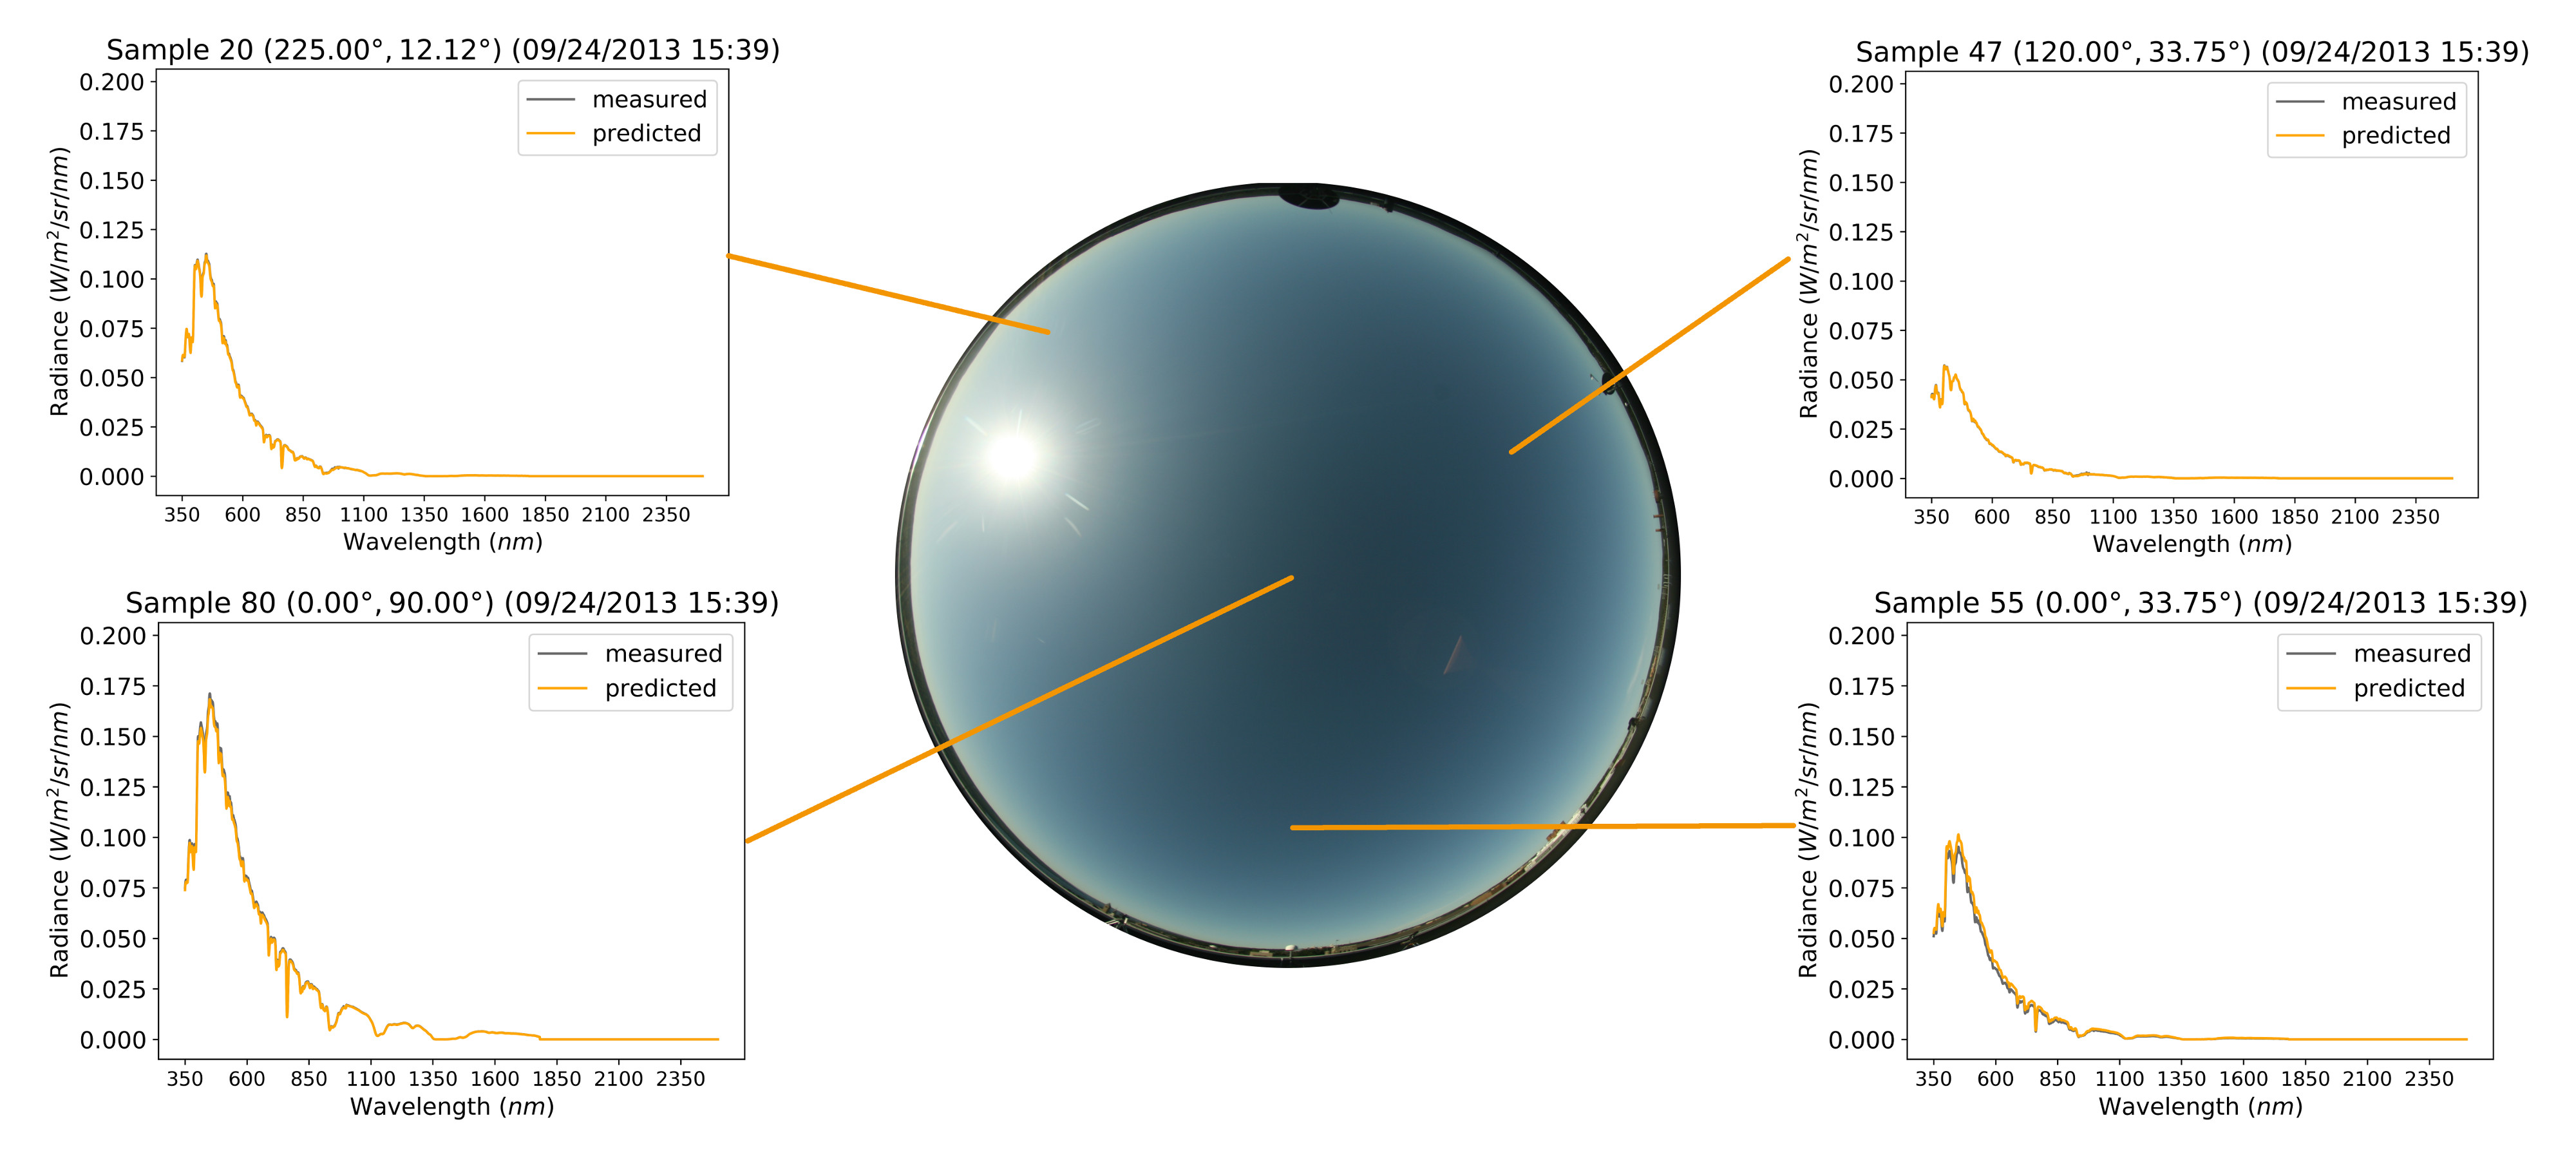
\includegraphics[width=1.0\textwidth]{img/09242013_samples.jpg}
\end{center}
\caption[errorcurves] { \label{fig:errorcurves}Select samples from clear sky capture 09/24/2013 15:39 predicted with ETR model clear dataset. \\ Video 1.~~http://dx.doi.org/doi.number.goes.here}
\end{figure}

\begin{figure} [hbtp]
\begin{center}
\begin{tabular}{c}
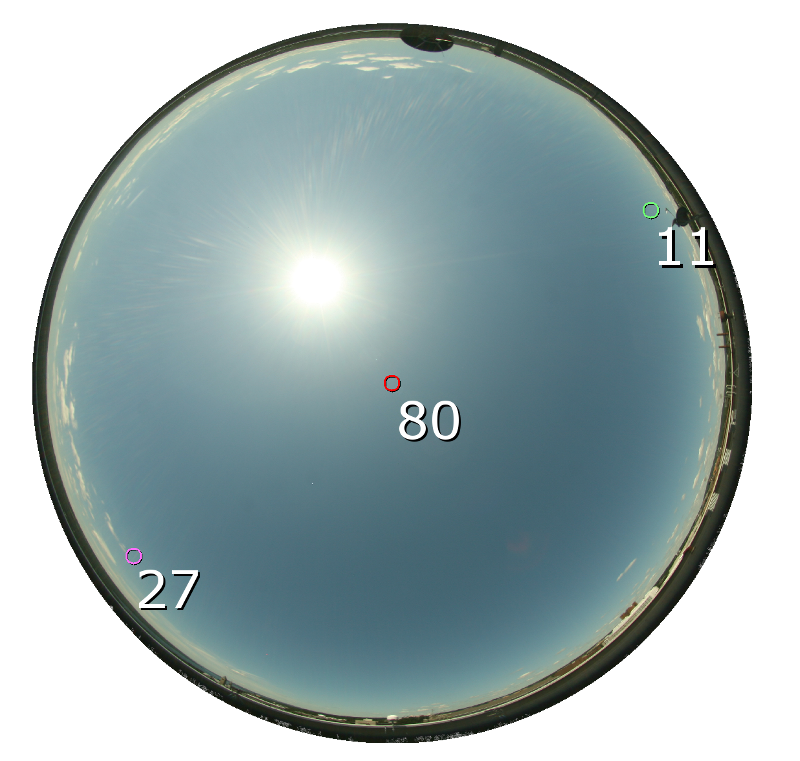
\includegraphics[width=0.44\textwidth]{img/results_072613_sky.png}
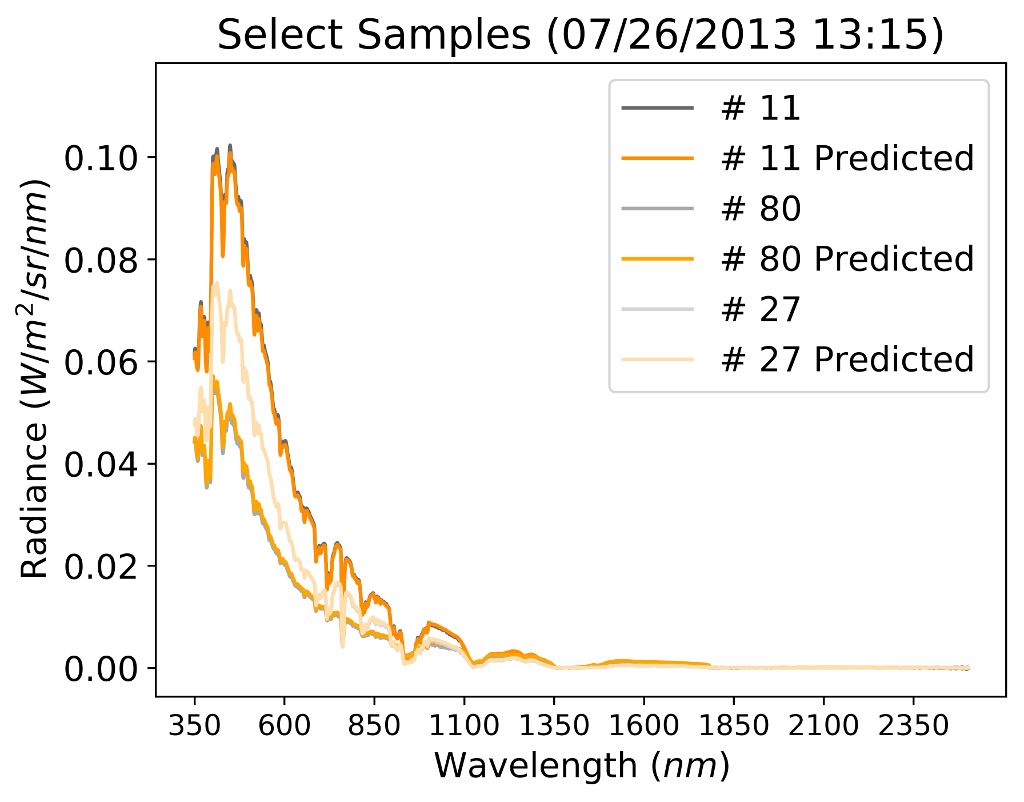
\includegraphics[width=0.54\textwidth]{img/results_072613_samples.png}
\end{tabular}
% \begin{tabular}{c}
% \includegraphics[width=0.24\textwidth]{img/results_predicted.jpg}
% \includegraphics[width=0.24\textwidth]{img/results_predicted.jpg}
% \includegraphics[width=0.24\textwidth]{img/results_predicted.jpg}
% \includegraphics[width=0.24\textwidth]{img/results_predicted.jpg}
% \end{tabular}
\end{center}
\caption[selectcurveratios] { \label{fig:selectcurveratios}Actual vs predicted radiance distributions for 3 select samples captured on 07/26/2013 13:15. Sample (80) is at the zenith, while (11) and (27) are near the horizon.}
\end{figure}

\begin{table}[hbtp]
\caption{Error metrics of actual vs predicted radiance curves for three select samples shown in Fig. \ref{fig:selectcurveratios} .}
\label{tab:selectcurveerrors}
\centering
\begin{tabular}{*{6}{c}}
    \\
    \toprule
    Sample Index & Coordinates & $\mathrm{R}^2$ & RMSD \\
    \midrule
    11 & $(123.75\degree,~12.1151\degree)$ & 99.97\% & 1.95\% \\
    27 & $(315.0\degree,~12.1151\degree)$ & 100.00\% & 0.57\% \\
    80 & $(303.75\degree,~90\degree)$ & 99.89\% & 1.92\% \\
    \bottomrule
\end{tabular}
\end{table}

\subsection{Whole Sky}

This work attempted to learn and predict collections of whole sky angular dependent radiance distribution curves for real-time application, because of the high demand across multiple disciplines for spectral illumination. Figs. \ref{fig:errorcurves}, \ref{fig:selectcurveratios}, and \ref{fig:wholesky} show that this is certainly possible with clear skies. All four holdout validation captures were predicted with success, three under 10\% error.

\begin{figure} [hbtp]
\begin{center}
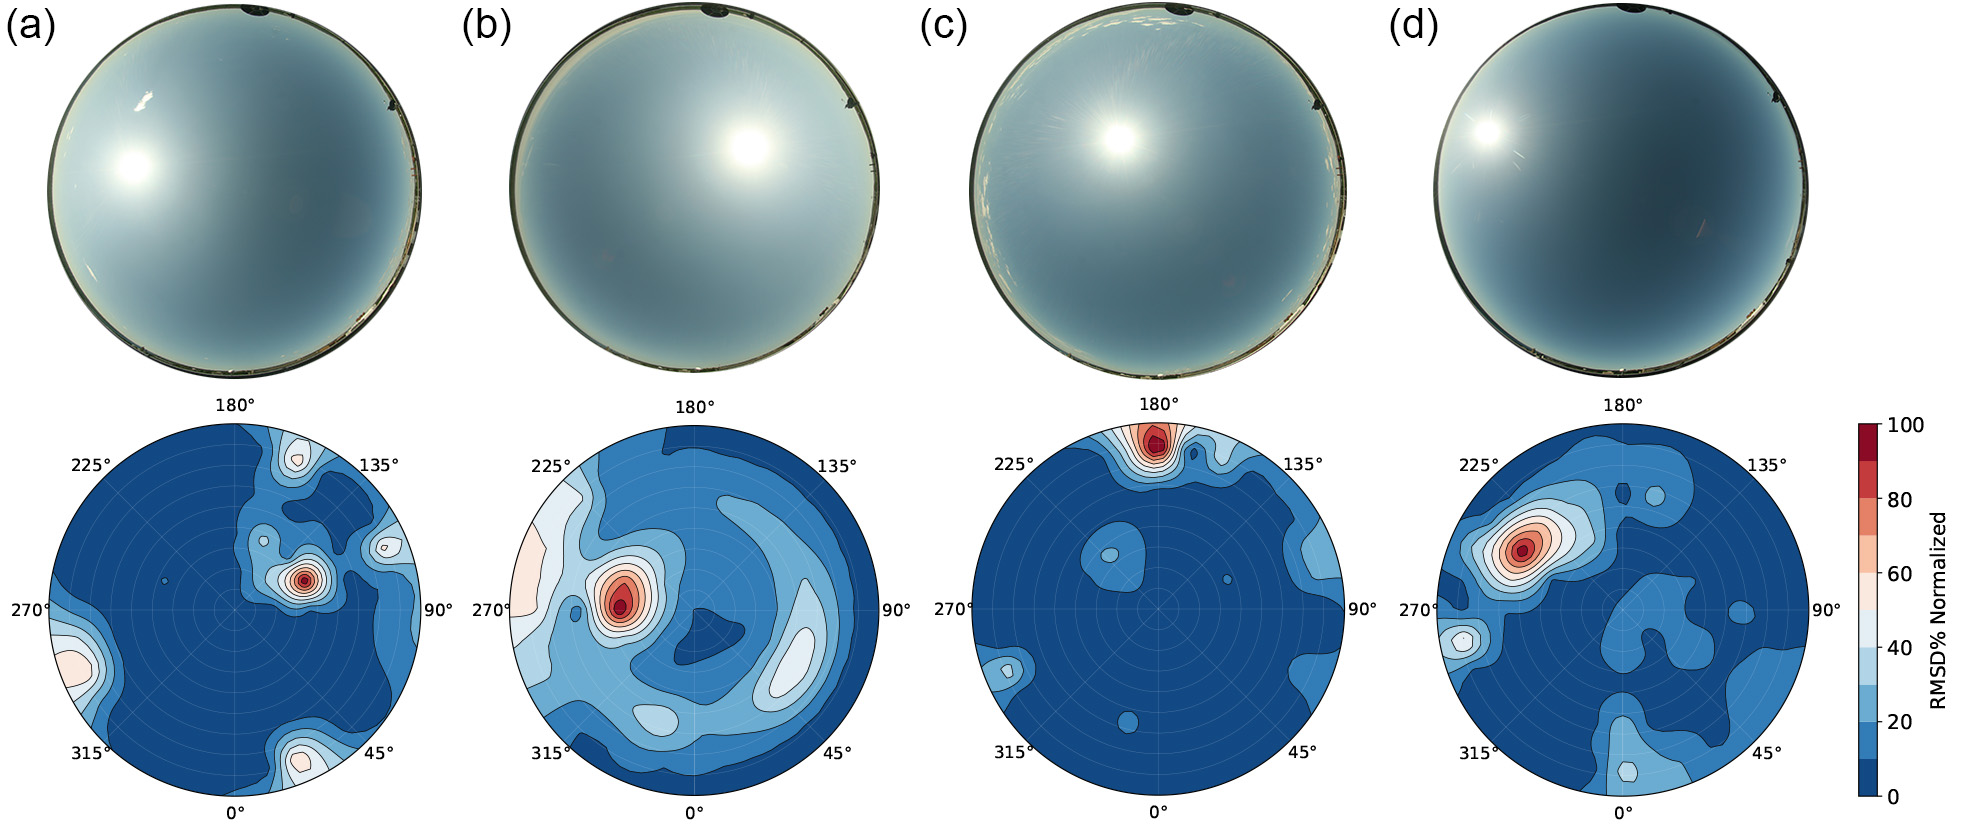
\includegraphics[width=1.0\textwidth]{img/results_wholeskyerrors.jpg}
\end{center}
\caption[wholesky] { \label{fig:wholesky}Demonstration of whole sky accuracy from holdout test data using ETR model trained on clear dataset. These captures correlate with overall error reported in Fig. \ref{fig:error_skies} and Tbl. \ref{tab:resultsETRclear}. This figure shows normalized RMSD\% for captures (a) 05/26/2013 15:15, (b) 05/27/2013 10:15, (c) 07/26/2013 13:15, and (d) 09/24/2013 15:39. We compare the generated spectral data with the captured data. (No samples from these captures were used for training.)}
\end{figure}

\section{Conclusions}
\label{sec:conclusions}

We set out to develop a machine learning method for estimating sky radiance distribution curves (including VIS, VNIR, and SWIR spectra) from images captured with a hemispherical commercial digital camera. We feel this project was a success in that regard. There is still much room for future work to greater improve accuracy for cloudy and mixed sky conditions, such as: tuning the RFR model, integrating turbidity and cloud type data from remote sensed sources like the GOES satellites, interpolating radiance curves for any point of a skydome, looking at the optimal non-linear regression for different channels across different color spectra (HLS, HSV, etc.), using PZA, SZA and SPA angles instead of (or in addition to) sky coordinates, taking advantage of our HDR data, investigating many other ML approaches (ANNs, etc.).

We hope this work will set the stage for future interdisciplinary research questions and experiments to help improve building energy simulation, photovoltaic placement, spectral rendering applications, etc. Having an online system that provides real-time whole sky angular spectral radiance distributions will improve real-time control systems. 

%And a recurrent learning method could even be employed to improve models while they are in use.

%Certainly more clear sky and color variation is desired. A great experiment would be to merge a dataset of sky images and radiance measurements from across the world and train upon that. Sky sampling pattern can vary (perhaps beneficially) so long as training/testing samples are extracted from a normalized set of images and radiance measurements (i.e. color format, exposure, pixel kernel, radiance units, etc.).

%\acknowledgments
\section*{ACKNOWLEDGMENTS}
\label{sec:acknowledgements}

We would like to formally acknowledge Dr. Donald P. Greenberg and the Program of Computer Graphics (PCG) at Cornell University for their support during data capture and open source release of the sky data used for analysis in this project; Kevin Pratt, Hurf Sheldon, and Lars Schumann for helping build the sky scanner; Dr. William D. Philpot for many discussions on spectral measurements with the ASD FieldSpec device; Dr. Harold van Es for lending PCG the ASD spectroradiometer to conduct experiments; and Daniel Knowlton for the predecessor to our SkyDataViewer and work on the spectral sky project.

% references
\bibliography{citations} % bibliography data in report.bib
\bibliographystyle{spiebib} % makes bibtex use spiebib.bst
\end{document} 
